\documentclass[12pt,letterpaperpaper,]{book}
\usepackage{lmodern}
\usepackage{amssymb,amsmath}
\usepackage{ifxetex,ifluatex}
\usepackage{fixltx2e} % provides \textsubscript
\ifnum 0\ifxetex 1\fi\ifluatex 1\fi=0 % if pdftex
  \usepackage[T1]{fontenc}
  \usepackage[utf8]{inputenc}
\else % if luatex or xelatex
  \ifxetex
    \usepackage{mathspec}
  \else
    \usepackage{fontspec}
  \fi
  \defaultfontfeatures{Ligatures=TeX,Scale=MatchLowercase}
    \setmonofont[Mapping=tex-ansi,Scale=0.8]{Source Code Pro}
\fi
% use upquote if available, for straight quotes in verbatim environments
\IfFileExists{upquote.sty}{\usepackage{upquote}}{}
% use microtype if available
\IfFileExists{microtype.sty}{%
\usepackage[]{microtype}
\UseMicrotypeSet[protrusion]{basicmath} % disable protrusion for tt fonts
}{}
\PassOptionsToPackage{hyphens}{url} % url is loaded by hyperref
\usepackage[unicode=true]{hyperref}
\hypersetup{
            pdftitle={DRAFT Dissertation Prospectus},
            pdfauthor={Danton Noriega},
            pdfborder={0 0 0},
            breaklinks=true}
\urlstyle{same}  % don't use monospace font for urls
\usepackage[margin=1in]{geometry}
\usepackage{natbib}
\bibliographystyle{apalike}
\usepackage{longtable,booktabs}
% Fix footnotes in tables (requires footnote package)
\IfFileExists{footnote.sty}{\usepackage{footnote}\makesavenoteenv{long table}}{}
\usepackage{graphicx,grffile}
\makeatletter
\def\maxwidth{\ifdim\Gin@nat@width>\linewidth\linewidth\else\Gin@nat@width\fi}
\def\maxheight{\ifdim\Gin@nat@height>\textheight\textheight\else\Gin@nat@height\fi}
\makeatother
% Scale images if necessary, so that they will not overflow the page
% margins by default, and it is still possible to overwrite the defaults
% using explicit options in \includegraphics[width, height, ...]{}
\setkeys{Gin}{width=\maxwidth,height=\maxheight,keepaspectratio}
\IfFileExists{parskip.sty}{%
\usepackage{parskip}
}{% else
\setlength{\parindent}{0pt}
\setlength{\parskip}{6pt plus 2pt minus 1pt}
}
\setlength{\emergencystretch}{3em}  % prevent overfull lines
\providecommand{\tightlist}{%
  \setlength{\itemsep}{0pt}\setlength{\parskip}{0pt}}
\setcounter{secnumdepth}{5}
% Redefines (sub)paragraphs to behave more like sections
\ifx\paragraph\undefined\else
\let\oldparagraph\paragraph
\renewcommand{\paragraph}[1]{\oldparagraph{#1}\mbox{}}
\fi
\ifx\subparagraph\undefined\else
\let\oldsubparagraph\subparagraph
\renewcommand{\subparagraph}[1]{\oldsubparagraph{#1}\mbox{}}
\fi

% set default figure placement to htbp
\makeatletter
\def\fps@figure{htbp}
\makeatother

\usepackage{booktabs}
\usepackage{lscape}
\usepackage{longtable}
\usepackage{bm}
\usepackage{isomath}
\usepackage{setspace}
% \doublespacing
\usepackage[bf,singlelinecheck=off]{caption}
\newcommand{\matr}[1]{\mathbf{#1}}
\newcommand{\blandscape}{\begin{landscape}}
\newcommand{\elandscape}{\end{landscape}}

\setromanfont[Mapping=tex-text]{Minion Pro}
\setsansfont[Mapping=tex-text]{Source Sans Pro}
\setmonofont[Mapping=tex-text,Scale=0.8]{Source Code Pro}

\usepackage{framed,color}
\definecolor{shadecolor}{RGB}{248,248,248}

\renewcommand{\textfraction}{0.05}
\renewcommand{\topfraction}{0.8}
\renewcommand{\bottomfraction}{0.8}
\renewcommand{\floatpagefraction}{0.75}

% \renewenvironment{quote}{\begin{VF}}{\end{VF}}
\let\oldhref\href
\renewcommand{\href}[2]{#2\footnote{\url{#1}}}

\ifxetex
  \usepackage{letltxmacro}
  \setlength{\XeTeXLinkMargin}{1pt}
  \LetLtxMacro\SavedIncludeGraphics\includegraphics
  \def\includegraphics#1#{% #1 catches optional stuff (star/opt. arg.)
    \IncludeGraphicsAux{#1}%
  }%
  \newcommand*{\IncludeGraphicsAux}[2]{%
    \XeTeXLinkBox{%
      \SavedIncludeGraphics#1{#2}%
    }%
  }%
\fi

\makeatletter
\newenvironment{kframe}{%
\medskip{}
\setlength{\fboxsep}{.8em}
 \def\at@end@of@kframe{}%
 \ifinner\ifhmode%
  \def\at@end@of@kframe{\end{minipage}}%
  \begin{minipage}{\columnwidth}%
 \fi\fi%
 \def\FrameCommand##1{\hskip\@totalleftmargin \hskip-\fboxsep
 \colorbox{shadecolor}{##1}\hskip-\fboxsep
     % There is no \\@totalrightmargin, so:
     \hskip-\linewidth \hskip-\@totalleftmargin \hskip\columnwidth}%
 \MakeFramed {\advance\hsize-\width
   \@totalleftmargin\z@ \linewidth\hsize
   \@setminipage}}%
 {\par\unskip\endMakeFramed%
 \at@end@of@kframe}
\makeatother

\newenvironment{rmdblock}[1]
  {
  \begin{itemize}
  \renewcommand{\labelitemi}{
    \raisebox{-.7\height}[0pt][0pt]{
      {\setkeys{Gin}{width=3em,keepaspectratio}\includegraphics{images/#1}}
    }
  }
  \setlength{\fboxsep}{1em}
  \begin{kframe}
  \item
  }
  {
  \end{kframe}
  \end{itemize}
  }
\newenvironment{rmdnote}
  {\begin{rmdblock}{note}}
  {\end{rmdblock}}
\newenvironment{rmdcaution}
  {\begin{rmdblock}{caution}}
  {\end{rmdblock}}
\newenvironment{rmdimportant}
  {\begin{rmdblock}{important}}
  {\end{rmdblock}}
\newenvironment{rmdtip}
  {\begin{rmdblock}{tip}}
  {\end{rmdblock}}
\newenvironment{rmdwarning}
  {\begin{rmdblock}{warning}}
  {\end{rmdblock}}

\usepackage{makeidx}
\makeindex

\urlstyle{tt}

\usepackage{amsthm}
\makeatletter
\def\thm@space@setup{%
  \thm@preskip=8pt plus 2pt minus 4pt
  \thm@postskip=\thm@preskip
}
\makeatother

\title{DRAFT Dissertation Prospectus}
\author{Danton Noriega}
\date{February 27, 2017}

\begin{document}
\maketitle

\setlength{\abovedisplayskip}{-5pt}
\setlength{\abovedisplayshortskip}{-5pt}
\mainmatter

{
\setcounter{tocdepth}{2}
\tableofcontents
}
\chapter*{Dissertation Overview}\label{dissertation-overview}
\addcontentsline{toc}{chapter}{Dissertation Overview}

Chapter 1 is an evaluation of the effectiveness of the Double Up Food
Bucks program. ``Effectiveness'' will be defined by the change in total
sales and volume of produce sold within 17 grocery stores that implement
Double Up (treatment group). The control group comprises 15 stores where
Double Up was not implemented. A difference-in-differences and
regression discontinuity design will be used to measure the size of the
effect.

Improving health and food equity of SNAP participants is the broader
policy concern. The mechanism is a financial incentive---Double Up Food
Bucks---designed to increase fruit and vegetables consumption. A
comparison will be made with another financial incentive program called
the \emph{Healthy Incentives Pilot} (HIP). I will argue how and why an
evaluation of the Double Up program is an important addition to the
current literature.

Chapter 2 extends the work of \citet{schenck-fontaine_use_2016}. Through
surveys, \citet{schenck-fontaine_use_2016} examine how families coping
with poverty and economic instability supplement their SNAP benefits
with additional assistance from informal and formal resources. In my
paper, I dig deeper into how and when families use additional formal
resources beyond SNAP---such as food banks and emergency cash
assistance. My aim is to provide a more detailed understanding of these
role formal networks play in supporting Durham families coping with
poverty.

Chapter 3 exploits the random assignment of the Durham Connects program
to measure its long term impact on social service applications. Durham
Connects (DC) provides free in-home nursing visits to residents of
Durham County. It was implemented as an RCT between July 2009 to
December 2010. The design treats DC as an information treatment. The DC
information treatment (e.g.~a nurse contact to ask questions and provide
assistance) is expected to lower the learning and barrier costs of low
income families with children when applying for social services.

\chapter{An Evaluation of the Double Up Food Bucks
program}\label{chapter-1}

\section*{Introduction}\label{intro-1}
\addcontentsline{toc}{section}{Introduction}

Chronic conditions like obesity, heart disease, and other metabolic risk
factors (stroke, type II diabetes, etc.) are estimated to cost the US
health care system between 200 to 400 billion dollars annually
\citep{cawley_medical_2012, chatterjee_checkup_2014}. More importantly,
these diseases account for hundreds of thousands of deaths each year.
Heart disease alone is the leading cause of death for all persons in the
US, with stroke fifth and diabetes seventh
\citep{national_center_for_health_statistics_health_2015}. Diet is
closely linked to these conditions, particularly obesity and
cardiovascular disease. There is strong evidence that a diet high in (1)
vegetables, fruits, nuts, unsaturated oils, fish, and poultry, but low
in (2) red and processed meat and sugar-sweetened foods and drinks,
helps lower body weight, blood pressure, and the risk of cardiovascular
disease
\citep{mente_systematic_2009, nutrition_evidence_library_series_2014}.
Improving the diet of Americans has therefore become an increasing
priority for the United States, especially for struggling families that
participate in the Supplemental Nutrition Assistance (SNAP) program.

SNAP is a federal aid program administered by the Food and Nutrition
Service (FNS), an agency of the U.S. Department of Agriculture (USDA).
At 74 billion dollars in FY2015 with roughly 45.8 million participants,
it is the largest food assistance program in the US
\citep{usda_fns_supplemental_2016}. To be eligible for SNAP, a household
must be sufficiently budget constrained that hunger is considered likely
without assistance. Eligibility is a function of countable resources,
vehicle ownership and value, household size, gross or net monthly
income, household composition, and meeting certain work
requirements.\footnote{For more details, visit
  \url{http://www.fns.usda.gov/snap/eligibility}} Some eligibility
requirements vary by state, but in general, a family with less than
\$2000 in countable resources, where the adults work at least part-time
earning a gross (net) monthly income at or below 130\% (100\%) of the
federal poverty line, is eligible to receive SNAP benefits. Aside from a
few restrictions---no alcohol, tobacco, non-food items, read-to-eat
meals, or hot foods---households can use SNAP benefits to purchase any
foods that will be prepared and consumed at home. Unfortunately, the
purchasing patterns of the average SNAP household are not conducive to a
healthy diet.

Research on the dietary patterns of households receiving SNAP benefits
has found that they are significantly \emph{less} likely to meet USDA
dietary guidelines than the average US household and much \emph{more}
likely to consume unhealthy foods
\citep{andreyeva_dietary_2015, nguyen_supplemental_2015, wolfson_fruit_2015}.
A smaller set of research has found that SNAP households, at best,
consume same amount of unhealthy foods (e.g.~sugar-sweetened beverages,
baked goods, snacks, candy, etc) compared to SNAP-ineligible households
\citep{todd_caloric_2014, hoynes_snap_2015}. In other words, SNAP
households consume foods that are less healthy or about the same as
SNAP-ineligible households. This is a concerning result given that most
US households, regardless of income, already purchase and consume far
too much meat and foods rich in sugars and fats, and far too few fruits,
vegetables and whole grains
\citep{usda_scientific_2015, frazao_high_1999}. However, the purpose of
SNAP is to keep struggling families from going hungry, not to ensure
they consume the best possible diet. SNAP is designed to act like cash,
helping families access more food than they could otherwise do so
without assistance \citep{hoynes_snap_2015}. It is therefore not a
failing of the SNAP program if benefits are used to purchase unhealthy
foods.

The SNAP program could be change such that it could continue satisfying
its role as an anti-hunger program while simultaneously encouraging
healthier purchases. \citet{blumenthal_strategies_2014} and
\citet{leung_qualitative_2013} both surveyed a field of stakeholders and
policy experts in the SNAP program about what they would do to improve
the dietary quality of purchases. In both studies, restricting the
purchase of unhealthy foods (e.g.~sugar-sweetened beverages) and
promoting healthy purchases through monetary incentives were the two
most popular improvements (i.e.~ranked the highest or most often
suggested).\footnote{It should be mentioned that there were other, less
  popular recommendations, such as modifying how SNAP benefits are
  distributed and improving nutrition education. For more details, see
  \citet{blumenthal_strategies_2014} and \citet{leung_qualitative_2013}}.

One common suggestion is to restrict the SNAP program to the same set of
eligible foods as the Woman, Infants, and Children (WIC) program
\citep{dinour_food_2007}. The WIC program provides food vouchers which
limit households to a select group of food products. These food products
are specifically selected to ensure women and their children receive
nutritious, healthy foods. In other words, the WIC program, by design,
places restrictions on food choices by defining a list of
\emph{eligible} items, as opposed to the SNAP program, which defines a
list of \emph{ineligible} items. Another common, and simpler, suggestion
is to expand the existing list of ineligible items (e.g.~alcohol) with
products that are unambiguously lacking in nutrition and easy to
identify, like soda or candy. New York City, for example, attempted to
ban the purchase of sugar-sweetened beverages, and the state of Maine
attempted to restrict the purchase of sodas, candy, and any other
taxable food items \citep{gundersen_snap_2015}. Both restrictions were
overturned by the USDA.

There are problems with ``improving'' the SNAP program by implementing
even greater purchasing restrictions. First, there is no reason to
believe that such a restriction would work. The restriction assumes
that, under WIC-like requirements, households will substitute healthy
foods for unhealthy foods when using SNAP benefits. What would most
likely happen is that households would shift to purchasing unhealthy
foods with cash. Second, such restrictions would likely lead to a drop
in SNAP participation \citep{gundersen_snap_2015}. Restricting choice is
a paternalistic policy that would further stigmatize SNAP participation.
It would give the impression that SNAP beneficiaries are assumed to have
worse diets and that they cannot be trusted to make healthy food
purchases. Participation would also drop due to increased transactions
costs of purchasing items with SNAP. Not all stores would clearly mark
which items were SNAP eligible nor should participants be expected to
remember. The result would be longer, more frustrating shopping trips.
Lastly, it is important to remember that for many SNAP recipients,
freedom of choice is what makes the SNAP program popular and easy to use
\citep{edin_snap_2013}.

The most popular ``improvement'' was providing a monetary incentive to
SNAP participants for purchasing healthy foods
\citep{blumenthal_strategies_2014, leung_qualitative_2013}. Monetary (or
financial) incentives, in this context, tend to be a rebate or voucher
awarded to SNAP households for using their benefits to buy certain
healthful foods, generally mineral-rich and nutrient-dense fruits and
vegetables (i.e.~leafy greens but not white potatoes). These monetary
incentives for buying ``targeted'' fruits and vegetables (aka TFVs) are
exclusive to SNAP participants. Much like a grocery stores loyalty card
or a student ID card, retailers can ``discriminate on price'' (aka
``target the incentive'') using SNAP Electronic Benefit Transfer (EBT)
cards to identifying eligible participants. Monetary incentives in the
food retail environment are popular for two main reason. First, the
framing of the ``improvement'' is positive. Instead of ``punishing''
SNAP participants through paternal restriction or disincentives (not
covered), monetary incentives reward participants for healthy shopping
behavior \citep{gundersen_snap_2015}. Retailers also prefer the positive
framing of monetary incentives. For the moment, monetary incentives
programs for SNAP participants are not wide spread. Therefore, taking up
an incentive program, assuming the cost of implementation isn't too
expensive, creates an opportunity for retailers to differentiate
themselves from their competitors \citep{hartmann_corporate_2011}. The
second reason is a strong theoretical framework established by
neoclassical economics supporting incentives as an effective mechanism
for changing human behavior. In practice, however, incentives have had
mixed results, but there is building evidence that incentives may work
in the food retail space.

How, why, and to what effect incentives may encourage SNAP participants
to purchase more targeted fruits and vegetables will be discussed in
detail below, and is the motivating question behind this paper.

\subsection*{Financial Incentives to Encourage Healthy Food
Purchases}\label{financial-incentives-to-encourage-healthy-food-purchases}
\addcontentsline{toc}{subsection}{Financial Incentives to Encourage
Healthy Food Purchases}

Encouraging healthy behavior through financial incentives has a long
history. Results are mixed. For example, financial incentives have been
shown to help individuals commit to regular exercise, improve dieting,
increase weight loss, and to quit smoking, but the intended effect of
the financial incentives were often only short-term (see
\citet{gneezy_when_2011} and \citet{cawley_economy_2015} for an
overview). \citet{gneezy_when_2011} also explain, through a review of
the literature, that depending on the context and design, incentives can
backfire, producing an effect known as ``crowd out''. Crowd out occurs
when an incentive displaces the intrinsic reward of a behavior
(originally defined for ``prosocial'' behavior, like volunteering or
giving blood; see \citet{benabou_incentives_2006}). The behavior then
becomes dependent on the extrinsic reward. As a result, having shifted
from being intrinsically rewarding to extrinsically rewarding, the
positive behavior continues only as long as the monetary incentive is
provided. More significantly, the intrinsic reward of the behavior does
not return once it has been ``crowded out''. Therefore, the long-term
effect of a monetary incentive can be negative, despite showing positive
effects in the short-term. That said, incentives can produce successful
long-term results if they are instead used as a mechanism to build good
habits. This requires that the incentives be salient and produce
immediate feedback without neglecting behavioral findings such as loss
aversion and mental accounting \citep{john_financial_2011}.

Given the research on incentives, it is reasonable to assume that a
monetary incentive for SNAP participants to purchase healthy foods, like
fruits and vegetables, may fail or even backfire. Should the act of
purchasing healthy foods be intrinsically rewarding to SNAP shoppers,
introducing an incentive may produce a ``crowd out'' effect. However,
recent field experiments find that incentives can establish healthy food
choice as a habit, possibly overriding any crowd out. Daily incentives
encourage children to make healthier food choices in school lunchrooms,
who in turn develop positive, long-term food habits
\citep{loewenstein_habit_2016, list_behavioralist_2015, belot_incentives_2014}.
Outside of the school lunchroom environment,
\citet{list_incentives_2015} found that similar habit formation is
possible with incentives in a more traditional food retail environment.
In their experiment, \citet{list_incentives_2015} provided an incentive
to 222 shoppers (\$1) to use their rewards cards, but then randomly
assigned each participant to the control group to one of three
interventions: \emph{information}, \emph{incentive}, or
\emph{combination}. The \emph{information} treatment was a flyer with
tips on how to prepare fruit and vegetable dishes as well as the health
benefits of eating more fruits and veggies. The \emph{incentive} was an
additional dollar for every 5 cups of targeted fruits and vegetables
(TFVs) purchased. The \emph{combination} treatment group included both.
The intervention lasted for 5 months but each group continued to be
observed for roughly 6 weeks months after. The \emph{information}
intervention had no effect, but the \emph{incentive} and
\emph{combination} interventions on average doubled their purchase of
fruits and vegetables in comparison to the control group. Most
promisingly, the gap persisted with minimal shrinkage for 6 weeks
following the end of the intervention. However, there was no follow up
after the 6-week post-intervention period. It is therefore possible the
gap closed over multiple months (as opposed to multiple weeks).

The design, food environment, and target of the incentive in each of
these experiments is important. First, the incentive in these
experiments is designed to be salient and immediate. In the school
lunchroom experiments, the children are aware of the incentive and
receive the reward (e.g.~a small token) immediately after selecting the
healthy food item. Likewise, the shoppers received their additional \$1
reward for every 5 cups of TFVs at checkout. One distinction between the
designs is frequency. The children are exposed to the incentive every
school day in the lunchroom experiments. The shoppers, on the other
hand, were exposed as frequently or as infrequently as they chose. This
distinction is important, as the latter better reflects the experience
of shoppers using the SNAP benefits. Second, the food environment is
important because it determines what choices are available. The children
have a finite set of options in the school lunchroom and they also have
no outside option (besides not eating lunch). The children optimize on a
relatively small set of choices and, for the duration of the
intervention, the incentive always existed. Food retail environments are
drastically different. There are numerous competing food choices and
generally other outside options.\footnote{It should be noted that this
  is not always the case. In \citet{list_incentives_2015}, for example,
  the store that was selected for the experiment was one of the few
  places local shoppers could find fresh produce. The store itself was
  located in one of Chicago's poorer neighborhoods.} It is substantially
more difficult for the shopper to optimize over such a large set of
choices. Last, and most obviously, one set of studies targets children,
the other adults. A priori, we would expect a monetary incentive to
affect children differently than adults. The fact that habit formation
through incentives appears possible for both target groups is promising.

Research where SNAP participants are the target group is nascent. The
USDA's Food and Nutrition Services (FNS) ran the first large scale
randomized control trial investigating the impact of a financial
incentive for targeted fruits and vegetables in 2011. The experiment was
called the Healthy Incentives Pilot (HIP). HIP is the precursor to every
incentive program currently being funding by the USDA. It also provides
the data for the few papers recently published on incentives for SNAP
participants.

\subsection*{The Healthy Incentives
Pilot}\label{the-healthy-incentives-pilot}
\addcontentsline{toc}{subsection}{The Healthy Incentives Pilot}

A brief overview of the Healthy Incentives Pilot is necessary to provide
context to, and contrast with, more recent financial incentive programs.

The UDSA's Food and Nutrition Services designed the Healthy Incentives
Pilot. The pilot was funded by the Food, Conservation, and Energy Act of
2008 to test whether financial incentives would increase consumption of
targeted fruits and vegetables (TFVs). SNAP participants were the target
group.

HIP was designed as a large scale randomized control trial (RCT). FNS
partnered with the Massachusetts Department of Transitional Assistance
to implement HIP. The pilot lasted from early 2011 to the end of 2012.
The population included all 55,095 SNAP participants in Hampden County,
MA. Hampden County is the poorest county in Massachusetts and has the
highest rates of obesity and other diet-related chronic illness
(e.g.~type 2 diabetes).

Of the 55,095 SNAP participants, 7,500 were randomly assigned to the
treatment group. The remainder fell into the control group. The
treatment was a 30 cent (or 30\%) rebate on every dollar spent on TFVs.
The rebate was capped at \$60 per month. To receive the rebate, selected
SNAP participants had to use their EBT cards at participating retailers.
The rebate, which was returned to their EBT account, could then be used
on any food item. That is, the rebate could only be earned buying TFVs,
but could be redeemed buying any SNAP eligible food item. Most HIP
participants spent about \$12 a month on TFVs, earning an average of
\$3.65 per month in rebates---drastically lower than the \$60 per month
rebate cap.

The evaluation was conducted using 24-hour dietary recall surveys. A
total of 5,000 participants were selected to be surveyed, even split
between treatment and control (2,500 HIP, 2,500 non-HIP). The first
survey was conducted prior to the start of the pilot. This established a
baseline. The second survey occurred 4 to 6 months in to the pilot and
the third survey occurred 9 to 11 months in. (The variation, e.g.~4 to 6
months, was due to the treatment being implemented in 3 waves of 2500.)

The evaluation found that the 30\% rebate lead to about a 26\% increase
in consumption of TFVs. This was equivalent to about 0.24 cups of TFVs.
Roughly 60\% of the increase was due to increased vegetable consumption
and 40\% due to increased fruit consumption. The effect, in absolute
terms (0.24 cups), seems small. But a \(0.87\) price elasticity,
relative to other results in the literature, is quite high---\(0.7\) and
\(0.48\), on average, for fruits and vegetables, respectively
\citep{andreyeva_impact_2010}.

Despite some limitations and technical problems---underreporting on the
24-hour recall survey and system glitches early in the pilot (see pages
60 and 208-210 of \citet{bartlett_evaluation_2014})---HIP was considered
to be an overall success
\citep{klerman_short-run_2014, olsho_financial_2016}. It implemented on
of the largest, most complex RCTs to isolate how incentives can increase
household consumption of TFVs. It also provided a feasible model for
nationwide expansion (assuming cost reductions due to economies of
scale; see \citet{an_nationwide_2015}).

HIP also provides a framework for understanding how a financial
incentive, expanded dramatically in one geographic area, could improve
TFV consumption. But, as noted in the final HIP report, one of the most
prominent retailers in Hampden County chose not to participate (page 61,
\citet{bartlett_evaluation_2014}). Its third-party processor decided it
was too difficult and too costly to implement the financial incentive on
its point-of-sale technology. This strategic behavior by the retailer,
which had a significant presence in Hampden County, impacted where
participants could use the incentive.

Most financial incentive programs work at the local level, expanding
non-randomly. We should anticipate certain retailers (firms) to behave
strategically when participating in any of these incentive programs.
Likewise, we should anticipate voluntary (non-random) self-selection by
SNAP beneficiaries into these financial incentives programs. To this
end, more research is needed to understand the impact of incentive
programs under \emph{real-world} conditions. HIP provided evidence that
incentive programs can work, but barring state-wide or nation-wide
adoption of point-of-sale financial incentives, we should expect growth
to occur organically under non-experimental conditions.

An example of such a financial incentive program for SNAP participants
is the Double Up Food Bucks program (DUFB or Double Up). The non-random
expansion and impact of this financial incentives program will remain
the focus of this paper

\subsection*{The Double Up Food Bucks
Program}\label{the-double-up-food-bucks-program}
\addcontentsline{toc}{subsection}{The Double Up Food Bucks Program}

The success of HIP paved the way for the Food Insecurity Nutrition
Initiative (FINI), established by section 4208(b) of the Agricultural
Act of 2014 (aka 2014 Farm Bill). FINI---a 100-million-dollar
initiative---in turn piloted numerous non-profit financial incentive
programs aimed at improving the diets of SNAP participants.

Of specific interest is Double Up Food Bucks (DUFB or Double Up), an
incentives-based program funded by FINI. In 2009, the non-profit
organization Fair Food Network (FFN) launched the Double Up Food Bucks
program in Detroit, Michigan. The intention of the program was to get
more low-income families visiting and participating in local Detroit
farmer's markets. The mechanism for increasing participation was a
dollar-for-dollar match of locally grown fruit and vegetable purchases.
This subsidy was accessible only to low-income families receiving SNAP
benefits, who could exchange up to \$20 of their benefits for a wooden
token that could be used on up to \$40 worth of locally grown produce.

The DUFB program was considered successful given it had expanded to more
than 150 farmer's markets in 2014 from just 5 farmer's markets in 2009.
SNAP benefits have been used more than 200,000 times to purchase fresh
produce, with more than 10,000 first time SNAP customers visiting
farmer's markets in 2013 alone \citep{fair_food_network_double_2014}.
The program is considered by Fair Food Network to be a ``three-fold''
win given that the program helps local low-income families buy more
fresh produce, provides new customers for local farmer's, and stimulates
the local food economy. Relative to farmer's markets in other states,
DUFB did seem to be bringing in substantially more SNAP dollars (\$1.7
million in Michigan versus \$307,000 in Illinois, the second largest).

A 5.17 million dollar FINI grant was awarded to Fair Food Network to
help it pilot three adjustments to the Double Up Food Buck program
\citep{usda_nifa_usda_2015}. First, FFN needs to test DUFB as a
year-round program in select locations instead of the current seasonal
format. Second, shift away from the token system to providing DUFB
electronically at point-of-sale. Third, the DUFB needs to expand from
farmer's markets into other retail environments, like supermarkets and
grocery stores.

Successful expansion into supermarkets and grocery stores is critical.
Approximately 80\% of all SNAP benefits in 2015 were used in
supermarkets or super stores \citep{usda_fns_snap_2016}. Less than 1\%
percent of SNAP benefits were used at local farmer's markets. The amount
of SNAP benefits used in local farmer's markets has increased since
2009, but no where near the growth necessary to reach the type of stores
most frequented by low-income families. If localized financial incentive
programs like DUFB are going to be considered one of the USDA's many
tools to increase food access and combat obesity, then they must be
successfully implemented and scaled across supermarkets and grocery
stores. Most importantly, incentive programs like DUFB must prove they
are effective in changing purchasing habits within supermarket/grocery
store food environments.

\subsection*{Double Up Food Bucks vs the Healthy Incentives
Pilot}\label{double-up-food-bucks-vs-the-healthy-incentives-pilot}
\addcontentsline{toc}{subsection}{Double Up Food Bucks vs the Healthy
Incentives Pilot}

There are notable differences between DUFB and HIP that make the
evaluation of DUFB more difficult. In short, HIP was implemented as an
RCT. DUFB implementation is not. Let's explore in greater detail.

HIP had substantially more participating stores, all within the same
county (Hampden County, MA). DUFB has fewer participating stores, spread
across many different counties, and across many different grocery store
chains. Therefore, the probability of a SNAP shopper in Hampden County
having walked into a HIP participating store was much higher than a SNAP
shopper walking into any DUFB participating retailer.

The incentive delivery mechanisms also differ. First, all SNAP
beneficiaries who shop at a DUFB participating store receive the benefit
automatically. In other words, SNAP households that patron a store with
DUFB receive the incentive regardless of their intentions or awareness
of the DUFB incentive. Therefore, evaluating DUFB has the added
difficulty of identifying which shoppers are optimizing in response to
DUFB, as opposed to shopping normally. In contrast, SNAP households
assigned to the HIP treatment group were made aware of incentive and
were eligible to use it (even if they didn't quite understand how the
incentive program worked --- see \citet{bartlett_evaluation_2014}).
Households in the control group were not aware of the incentive and were
not eligible to use it. And because participants were assigned, HIP
evaluators could identify treated participants from control
participants.

Second, the DUFB financial incentive is substantially larger but more
restrictive. The DUFB incentive is a dollar-for-dollar match of locally
grown produce purchases capped at \$20 per day. The matched dollars are
accrued as points on a store loyalty card. Existing points are then
automatically redeemed as dollars on \emph{any} fresh produce purchases,
not just locally grown produce. In comparison, the HIP financial
incentive was a return of 30 cents per dollar spent on TFVs which could
be spent on \emph{any} food item. That is, the DUFB incentive doubled
the purchasing power of every dollars spent on TFVs \emph{only for more
TFVs}; the HIP incentive increased the purchasing power of every dollars
spent on TFVs by 30\% \emph{for any SNAP eligible food item}.

Finally, the experimental designed of HIP allowed researchers to form a
causal interpretation of their results; the average treatment effect is
the same as the average treatment effect on the treated. Any difference
in the purchase and consumption of TFV between the treatment and control
groups could therefore be attributed to the incentive. This is not the
case for DUFB. However, HIP implementation is the exception. How DUFB,
and similar financial incentive programs are implemented, is the norm.
The contribution of this paper will be evaluating and understanding the
impact of DUFB, given that DUFB and similar programs are implemented in
the ``real-world'' (non-experimental conditions)

\subsection*{Evaluating Double Up Food Bucks in Non-experimental
Conditions}\label{evaluating-double-up-food-bucks-in-non-experimental-conditions}
\addcontentsline{toc}{subsection}{Evaluating Double Up Food Bucks in
Non-experimental Conditions}

DUFB's expansion and implementation into supermarkets and grocery stores
did not follow an experimental design. Fair Food Network searched for
local partners in the Detroit area willing to participate in DUFB. Not
all grocery stores, especially the smaller independent stores, had the
capacity to implement the point-of-sale technology necessary for the
incentive---even if FFN offered to help cover the upgrade costs. The
result is a self-selected group of stores participating in DUFB. This,
in some ways, parallels what occurred in HIP, where one of the largest
retailers decided integrating their point-of-sale systems to include the
incentive was too expensive. This type of strategic firm behavior is
important to consider, even if complicates the evaluation of an
incentive program like DUFB.

In the real world, stores seek to maximize profits and will opt to
participate only if they expect to profit. Similarly, individuals will
self-select into participating; participation is optional and more
likely to occur with well-informed and motivated SNAP shoppers.
Selection, in this case, is a feature, not a flaw, of such incentive
programs when implemented by non-profits or policy makers. The evidence,
thanks to HIP, exists that incentives can lead to an increase in
consumption. The goal of this paper is therefore to accurately measure
the effect of the DUFB on TFV purchases while taking the selection into
account. That effect can then be extrapolated forward, albeit weakly,
using the results of HIP, to measure changes in consumption.

Fair Food Network started testing and gathering data from grocery stores
implementing DUFB in 2014. One of FFN's largest partners, a Michigan
grocery retail and distribution company, piloted the program in 2 of its
stores in 2014. The company has since expanded to 5 stores in 2015 and
then to 17 of 62 stores in 2016. Rapid scaling was possible due to the
point-of-sale technology used by the company to implement DUFB across
its stores. It provides, to date, the best case study of a firm
strategically scaling DUFB across numerous grocery stores that span
different geographic areas and populations.

All transaction data from 2014 - 2016 will be provided for every store
that has, at any point, participated in DUFB. These data are complete
(i.e.~no records have been removed) and at the item level. A complete
set of data will also be provided from another 15 stores where DUFB was
not implemented.

Currently, no research exists evaluating DUFB, or similar incentive
programs, using a complete set of store transaction data. HIP, for
example, only had transactions records for SNAP EBT cards. Transactions,
should a different tender be used by the same individual, could not be
observed. Therefore, these data provide an unprecedented opportunity to
analyze how the DUFB financial incentive performs under real-world
conditions. This paper will be, to the best of my knowledge, the first
to perform an evaluation of a financial incentive, targeted at SNAP
participants, using a complete set of data, from multiple stores, across
multiple years, and collected under non-experimental conditions.

\newpage

\section*{Motivation}\label{motivation}
\addcontentsline{toc}{section}{Motivation}

\textbf{Research Question}

\begin{quote}
How effective is the DUFB financial incentive at increasing the fresh
fruits and vegetables purchased by SNAP shoppers within a grocery store
environment?
\end{quote}

\textbf{Hypothesis 1}: I expect a slight increase (1 - 2\%) in SNAP EBT
expenditures on fruits and vegetables (FVs) during the months the DUFB
incentive is active in the experimental stores (Aug - Dec). I expect the
effect will fade over time. I expect no significant differences in fruit
and vegetable expenditures during the months the incentive is not in
effect (Jan - July).

Note that the DUFB incentive is applied automatically to all SNAP
shoppers earning or redeeming DUFB points (covered in more detail in the
\protect\hyperlink{data-1}{Data Section}). Therefore, by default, all
SNAP shoppers at a DUFB store are technically ``participating''.
However, SNAP shoppers should be considered ``passive'' or ``active''
participants. ``Active participation'' would characterize shoppers
responding to the DUFB incentive; ``passive participation'' would
characterize shoppers who continue to shop as usual, despite
automatically redeeming points.

From prior implementations of the program, participation rates in
DUFB-like incentive programs can be low. In this case, I expect SNAP
shoppers to consist of mostly ``passive'' participants. Combined with
the fact that SNAP dollars account for less than 5\% of all spending in
these stores, I don't think there is a very large pool of SNAP
participants to draw from. As a result, the ``active'' participants, who
respond to the incentive and purchase more fruits and vegetables, will
consist of a small fraction of total FV spending. Therefore, to capture
this effect, it is necessary to focus purchases made by the targeted
group (SNAP households).

I expect awareness of the DUFB program for this particular grocery chain
appears to be low. This is includes both staff and the shoppers
themselves. I don't know if the corporate office, which selected and
implemented the DUFB incentive, clearly communicated or advertised the
DUFB program to store management/staff and customers. As a result, I
expect ``active'' participation rates to be low. I must be clear that
this is merely a hunch. I don't think there is a large profit motive
behind implementing this program for the retailer. I think it is an
opportunity to pretend to be doing some good and to have something which
reflects a positive corporate image. A survey of store staff and of some
customers to test this hunch would be great.

\textbf{Hypothesis 2}: If measurable, I expect spending increases to
occur within the first 3 weeks of each month, when most SNAP benefits
are distributed and consumed. I also expect week 4 for all stores,
regardless of DUFB participation, to be relatively similar.

Prior research finds that SNAP shoppers spend their benefits soon after
receiving them, generally in one large shopping trip
\citep{wiig_art_2009, damon_first_2013}. The grocery stores are located
in a state where benefits are disbursed every odd day of the month
between the 3rd and 21st, spanning the first 3 weeks of each month.
Therefore, by the 4th week, few unspent dollars will exists. Since the
DUFB incentive is only triggered by the use of SNAP benefits, SNAP
shoppers will be unable to make use of DUFB.

I expect that, were we to remove the 4th week of each month from all
stores, the DUFB effect size will increase. I do not anticipate to see
shoppers behave in strategic saving behavior of DUFB points (which is
quite difficult given the automatic accrual and redemption system) nor
do I think FV spending to increase much without the presence of the
incentive. More importantly, since I cannot track link purchases to
individuals (more on this later), it will be impossible to identify
which transactions are made by SNAP shoppers when they are not using
their SNAP EBT cards.

\newpage

\hypertarget{data-1}{\section*{Data Description}\label{data-1}}
\addcontentsline{toc}{section}{Data Description}

These data come from a large grocery distributor and retailer serving
multiple grocery chains. Three years of data will be made available,
2014 through 2016. To my understanding, this includes months where the
DUFB incentive is active (Aug 1 to Dec 31) and inactive (Jan 1 to July
31) across all stores. These data are transaction level data and will
include (at least) store number, register, transaction ID, date and time
of purchase, payment type, item, dollars, and quantity.

Double Up implementation was considered for a single grocery chain. The
chain has more than 60 stores, 17 of which were selected as
``treatment'' stores (with Double Up). Of the remaining stores, data is
being made available from an addition 15 to serve as ``controls''. The
quotes here signify that these terms will be used as shorthand, but the
terminology is somewhat misleading. The use of ``treatment'' and
``control'' could lead one to think store assignment was random. It was
not.

{[}MISSING real specific details about the data e.g.~total transactions
observed etc.{]}

\subsection*{How the DUFB Incentive is
Implemented}\label{how-the-dufb-incentive-is-implemented}
\addcontentsline{toc}{subsection}{How the DUFB Incentive is Implemented}

The DUFB incentive can differ in implementation. Three different
implementations have been observed: earn/redeem DUFB points via loyalty
card, single-use paper coupon, and immediate discount. The earn/redeem
DUFB point system is unique to the retailer that provided these data.
For information on the other two DUFB implementations, see
\citep{margaret_schnuck_doubling_2016}.

The DUFB implementation for this particular grocery store chain is a
point system. SNAP shoppers can \emph{earn} points by buying locally
grown produce using their SNAP EBT card and their loyalty card. The
loyalty card is required because it is used to store and track earned
DUFB points. Each dollar spent buying locally grown produce earns a DUFB
point. SNAP shoppers are eligible to receive up to \$20 dollars worth of
DUFB points (20 points) per day. Earned points are not reflected
immediately on loyalty cards. They are redeemable the day after.

Points can be redeemed on \emph{any} eligible produce (excludes frozen
and canned fruits and vegetables). Any form of payment can be used when
redeeming points; it is not necessary to use a SNAP EBT card to redeem
points.

There are four important details about this implementation of the DUFB
incentive. I already mentioned the first but it is worth reiterating:
earned points take a day to be processed on a loyalty card. This forces
SNAP shoppers to delay the reward of the DUFB incentive earned by at
least a day. While perhaps a technological necessity (it takes time to
process and reflect earned points on loyalty card accounts), this delays
the transactional utility that could potentially be earned by the SNAP
shopper \citep{thaler_mental_1985}. I expect that delaying the
transactional utility reduces the ``pleasure'' and effectiveness window
of the DUFB incentive. SNAP shoppers tend to spend benefits in one large
shopping trip soon after receiving monthly benefits. These shopping
trips therefore correspond to the single largest opportunity to earn
DUFB points. Unless the shoppers returns to the store frequently to buy
fresh produce, the ``reward'' of redeeming points.

Second, the incentive alternates between earning and redeeming states. A
loyalty card with a DUFB point balance of zero is in an ``earning''
state. However, once DUFB points are earned by buying \emph{locally}
grown fresh produce, the card switches to a ``redeeming'' state; loyalty
cards with a point balance greater than zero will redeem until the point
balance is once again zero. This removes the possibility of
strategically ``banking'' earned points to be redeemed all at once (say
for a holiday shopping trip). Should I purchase \$10 dollars of local
produce and earn 10 points, the next time I purchase \emph{any} produce
(even local produce), my purchases will be redeemed from the point
balance until the 10 points are gone.

Third, the points \emph{earned} are not communicated to the shopper at
the moment of sale \citep{family_fare_double_2016}. In other words, the
fact that shoppers are earning points is \emph{not salient}. There is no
feedback connecting the purchase of fresh healthy produce to the fact
that the shopper is earning points. Currently available points (those
processed in prior shopping trips) are printed at the bottom of each
receipt, and can even be checked on-line or on in-store kiosks. But no
feedback or information is shared to the shopper during the current
sale. Earning points, at least, ends up being like any other shopping
trip. I would argue this is more a con than a pro. Certainly a bell
shouldn't ring when SNAP shoppers earn points. One of the great
consequences of moving to an EBT card is that the potential stigma of
using food stamps has greatly diminished. But shoppers could benefit
from some sort of feedback that is informative without producing a
spotlighting effect. For example, shoppers could be told, ``You saved
\$4.50 today and you also earned 5 DUFB points''.

{[}\textbf{I need to confirm that this does not happen}. Considering the
points earned don't appear on receipt, I do not see how the clerk know
to inform the customer. Does it appear on the machine?{]}

The fourth, and most important point, is the automatic earning and
redeeming of DUFB points. This implies the incentive works only if
individuals choose to actively participate in the program. This is
distinct to standard experimental procedure where individuals are
assigned to the treatment or control group and then choose to
participate (or not).

\subsubsection*{\texorpdfstring{What is a ``participant'' for this DUFB
implementation?}{What is a participant for this DUFB implementation?}}\label{what-is-a-participant-for-this-dufb-implementation}
\addcontentsline{toc}{subsubsection}{What is a ``participant'' for this
DUFB implementation?}

How a participant responds to assignment is generally referred to as
\emph{compliance} \citep{angrist_mostly_2008}.\footnote{Participants can
  be further categorized into ``compliers'', ``never-takers'',
  ``always-takers'', and ``defiers''. These categorizations provide
  useful terminology but are not relevant in the context of the DUFB
  incentive.} But in this case, it is the stores, not the individual
shoppers, that have been ``assigned'' to a treatment or control group.
Stores, if assigned to the treatment group by the retail chain, are
``compliers'' by default; the DUFB incentive is implemented on store's
point-of-sale (POS) system. Some stores (4) behaved somewhat like
``always-takers'', having asked to participate in DUFB, but most store
(13) are ``compliers''.\footnote{I must note that, while this creates
  some worries of ``self-selection'' by stores, I think this bias can be
  handled by a model that includes a store-level fixed-effect.}

How, then, does one think about SNAP shopper participation in the DUFB
program if it is stores that are ultimately assigned to the DUFB
program? SNAP shoppers have the option to benefit from the program
without ever being ``assigned'' to any treatment group. A shopper's
active participation in DUFB is therefore driven by another type of
self-selection. I imagine use of the DUFB incentive depends on a series
latent variables corresponding to individual shoppers, stores, and the
retail chain. For example, demographics, price sensitivity, food
preferences, health consciousness are all latent variables that could
affect shopper DUFB activity. Other latent variables include how
effectively the retail chain markets the DUFB program to management of
participating stores and how effectively this information is relayed by
stores to individual shoppers. Management's enthusiasm for the program
is likewise a latent retail chain and store-level variable.

Automatically redemption of the DUFB points also complicates identifying
individual participation. Automatic redemption of DUFB ``points'' means
I cannot identify which SNAP transactions are responding to the
incentive versus ``shopping as usual''. That is, I will observe many
SNAP transactions earning or redeeming DUFB points for fruits and
vegetables that are oblivious to the existence of the incentive. I will
also observe individuals who have chosen to actively participate in the
program. In aggregate, however, I assume that any increase in the total
amount of fruit and vegetables purchases in DUFB stores can be
attributed to the incentive. This is where having purchasing data from
the non-DUFB stores is important. The non-DUFB stores will help improve
estimation by controlling for any changes in fruit and purchases that
may occur for reasons other than the DUFB incentive e.g.~seasonal or
macroeconomic conditions.

\subsection*{Purchases Cannot Be Linked to Individuals (No Loyalty Card
Data)}\label{purchases-cannot-be-linked-to-individuals-no-loyalty-card-data}
\addcontentsline{toc}{subsection}{Purchases Cannot Be Linked to
Individuals (No Loyalty Card Data)}

One important variable that will not be made available is a variable for
loyalty card numbers. The company's use of loyalty cards across its many
chains was an exciting prospect. Previous transaction data from smaller
independent grocery chains had no way linking purchases to a single
unique identifier over time because these smaller chains did not have
advanced point-of-sale systems.

In earlier conversations with the company, it was understood that
loyalty cards would be made available. However, months into working with
the company, I was informed that this was no longer possible. Per the
company's legal department, the company cannot share any personal
information about their customers. Unfortunately for us, in the loyalty
card contract signed by customers, the loyalty card number itself is
considered personal information, meaning loyalty card numbers fall under
the same legal category as phone numbers and home addresses.

\subsection*{DUFB Incentive Inconsistency Across
Years}\label{dufb-incentive-inconsistency-across-years}
\addcontentsline{toc}{subsection}{DUFB Incentive Inconsistency Across
Years}

The retail company informed us that the way the DUFB incentive worked in
2016 is distinct from 2014 and 2015. The DUFB incentive in 2016 worked
by earning points for each dollar spent on \emph{locally grown} fresh
produce. (Recall that each point is equal to one dollar.) Points are
then redeemed automatically on \emph{any} fresh produce. However, in
2014 and 2015, the incentive was the \emph{opposite}. In those two
years, the DUFB incentive worked by earning points on \emph{any} fresh
produce, automatically redeeming points on \emph{locally grown} fresh
produce.

This is important because \emph{locally grown} fresh produce is a much
smaller subset of the \emph{any} fresh produce. Therefore, in years 2014
and 2015, shoppers could easily earn points but had a constrained set of
produce on which to redeem points. In any case, estimates of the
incentive for the year 2015 cannot be compared to estimates in the year
2016.

\subsection*{Limited Dependent
Variable}\label{limited-dependent-variable}
\addcontentsline{toc}{subsection}{Limited Dependent Variable}

It is very likely that for any recorded visit to the cashier---what I
call a ``transaction''---a customer does not purchase fresh fruits or
vegetables (FV). If I split a customer's items purchased during a
transaction into a few general categories (e.g.~dairy, candy, meat,
etc.) and aggregated expenditure over these categories, I will observe a
non-trivial amount of zeros. More importantly, these are ``true'' zeros
aka \emph{corner solutions}. That is, these zeros are not substitutes
for missing data or representing negative values but the result of a
utility-maximizing choice.

These concerns are covered in greater detail in the
\protect\hyperlink{methods-1}{Methods Section}.

\subsection*{Other Information}\label{other-information}
\addcontentsline{toc}{subsection}{Other Information}

\textbf{Past Experience with Similar Data}

This is not my first experience working with transaction data. At this
point, I have more than 3 years working with transaction data.
Furthermore, this is not my first experience with transaction data where
(1) DUFB was implemented and (2) transactions were not linked to
individuals.

I performed an analysis in April of 2016 for FFN using 5 months of
transaction data from 3 small Detroit-area grocery stores. Figure
\ref{fig:trx-cycle} was produced with those data. It was easy to
distinguish when SNAP benefits were being used in those data. Likewise,
it was easy to tell when transaction made use of the DUFB incentive
(either an issuing of DUFB or a redemption). A simple aggregation could
determine the total amount of dollars spent per some unit time
(\emph{day} was the smallest possible unit of time). I expected data for
my prospectus will be very similar. The empirical models in the next
section were developed under these expectations of the data.

\textbf{SNAP Spending is Cyclical}

In some prior work, I've observed that SNAP spending is cyclical,
peeking in the 2nd week. This is due to the state's monthly SNAP
benefits transfer schedule. Benefits are distributed every odd day of
the month between the 3rd and 21st. Each day maps to the digits
\texttt{0} through \texttt{9}. SNAP participants receive their benefits
once a month on the day corresponding to the last digit of their SNAP ID
number. For example, ID numbers that end in \texttt{0} receive their
benefits on the 3rd of each month. SNAP EBT benefits are spent quickly.
As a result, there are always fewer SNAP purchases during the 4th week
of the month. And fewer SNAP benefits means fewer transaction capable of
receiving the DUFB incentive. I'm not yet sure what impact this will
have on my analysis this time around, but I thought it important and
interesting to point out and consider.

\begin{figure}

{\centering 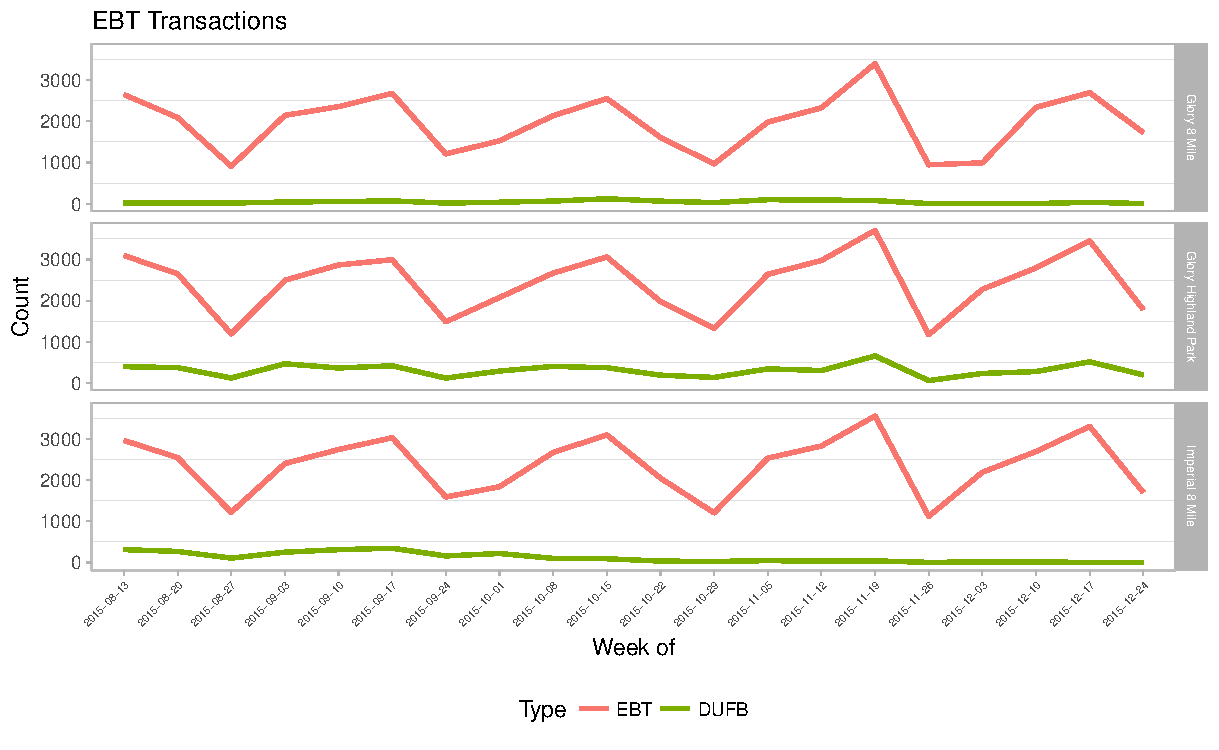
\includegraphics{figures/trx_counts} 

}

\caption{Example of how SNAP EBT benefits are spent in a predicable, week-to-week, cycle. It is the result of how benefits are distributed (uniformly across the first 3 weeks) and of how most SNAP participants spend their benefits (quickly and soon after being received). The red line is the count of transactions where SNAP EBT benefits were used as tender. Ignore the green line.}\label{fig:trx-cycle}
\end{figure}

The week-to-week cyclical pattern of SNAP EBT spending can be observed
in Figure \ref{fig:trx-cycle}. (Note that these are from a different
data source and different store chain, but from the same US state.) At
the start of the each month, SNAP EBT transactions (red line) increase
until peeking at the second week. The count then declines steadily
through the 4th week before once again spiking during the 1st week of
the following month. (Ignore the green line; these are DUFB counts from
a different data set.)

\textbf{Supply Chain Concerns}

One concern I had was if local supply of produce differed geographically
across the state where the stores are located. The company
representative told me that should not be a factor because all stores
are supplied from the same warehouse. Therefore, in theory, each store
should have the same local produce. I plan to visit the stores on a
later date to confirm that this is actually the case.

\hypertarget{store-selection-1}{\section*{Overview of Store Selection
and Expansion}\label{store-selection-1}}
\addcontentsline{toc}{section}{Overview of Store Selection and
Expansion}

How the 17 ``treatment'' stores and 15 ``control'' stores were selected
in 2016 is important. First and foremost, selection was \emph{not}
random. Stores were either selected by the company (13 of 17) or
self-selected into Double Up (4 of 17). Second, the 15 control stores
were selected \emph{after} the selection of the 17 treatment stores.
Data from all remaining stores was requested but the request was denied;
only 15 stores had been approved by the company's management. Finally,
and most importantly, the selection criteria for the 17 treatment stores
is \emph{observable}. The implications of this will be covered in more
detail in the \protect\hyperlink{methods}{Methods} section.

\subsection*{Selection and Expansion of Double Up
Stores}\label{selection-and-expansion-of-double-up-stores}
\addcontentsline{toc}{subsection}{Selection and Expansion of Double Up
Stores}

The first 2 stores were piloted with Double Up in 2014. Both were in
geographically distinct areas (these will be referred to as
``\texttt{Node\ 0}'' and ``\texttt{Node\ 1}''). There was a small
expansion adding 3 more stores in 2015. The 3 stores were selected
because they were geographically close to the 2 original pilot stores (2
close to \texttt{Node\ 0}, 1 close to \texttt{Node\ 1}). The 5 stores
are referred to as the ``core''. The location of these 5 stores,
separated in two clusters, established the geographic constraints that
were then used to determine most of the additional stores in 2016.

Double Up was expanded to 12 more stores in 2016, totaling 17. Of those
12, 6 were selected due to their proximity to the 5 core stores, their
SNAP EBT\footnote{Electronic Benefit Transfer.} sales figures, and
similarity in surrounding demographics (high population density, more
African-American). In other words, 9 of the 17 stores---excluding the
initial 2 pilot stores-----were selected on a set of \emph{observable}
characteristics. The remaining 6 stores were not.

Of the remaining 6 stores, 4 asked if they could be included in the
program. These stores \emph{self-selected} into Double Up, making these
stores fundamentally distinct. They were considered, and then included,
only because they fell within the ``Top 50''. The final 2 stores were
selected by the company for ``strategic business decision''. The best
interpretation of this is that the company thought that Double Up would
provide a competitive edge to the 2 included stores given some internal
calculus. How the company came to this decision is \emph{unknown} and
therefore \emph{unobserved}.

Table \ref{tab:store-class} helps understand the year by year expansion
of Double Up. Stores are classified as either \texttt{assigned},
\texttt{self-selected}, or \texttt{unobserved}. To be \texttt{assigned}
means a stores participation in Double Up was determined (assigned) by
the company; \texttt{self-selected} means the store asked the company to
participate; \texttt{unobserved} means that the company selected the
store to participate in Double Up but for unknown and unobserved
reasons. Numbers were assigned to each store for easy reference but
otherwise have no meaningful interpretation.

\begin{table}

\caption{\label{tab:store-class}Year by Year Store Selection. Stores 1 and 2 represent the initial 2014 pilot stores.}
\centering
\begin{tabular}[t]{rlll}
\toprule
Store & 2014 & 2015 & 2016\\
\midrule
1 & pilot & pilot & pilot\\
2 & pilot & pilot & pilot\\
3 &  & assigned & assigned\\
4 &  & assigned & assigned\\
5 &  & assigned & assigned\\
\addlinespace
6 &  &  & assigned\\
7 &  &  & assigned\\
8 &  &  & assigned\\
9 &  &  & assigned\\
10 &  &  & assigned\\
\addlinespace
11 &  &  & assigned\\
12 &  &  & self-selected\\
13 &  &  & self-selected\\
14 &  &  & self-selected\\
15 &  &  & self-selected\\
\addlinespace
16 &  &  & unobserved\\
17 &  &  & unobserved\\
\bottomrule
\end{tabular}
\end{table}

\subsection*{Expansion on Observables}\label{expansion-on-observables}
\addcontentsline{toc}{subsection}{Expansion on Observables}

An example expansion on \emph{observables} (using fake data) can be seen
in Figure \ref{fig:dufb-expansion}. In the top frame, one can see two
blue dots. These blue dots simulate the first two pilot stores in 2014.
The left blue dot is \texttt{Node\ 0} and the right blue dot is
\texttt{Node\ 1}. The gray zones represent areas of higher population
density. Dark gray is considered \emph{urban}, defined as having a
population density of 1500 persons or more per square mile. The light
gray are small towns and cities, more densely populated than very rural
areas, but could not be considered \emph{urban}. The expansion in 2015
(middle frame) proceeds to the stores closest to the original pilot
stores. The expansion continues to 6 more stores in 2016 (bottom frame)
away from the nodes but also along areas of higher population density.

Not conveyed in Figure \ref{fig:dufb-expansion} is that the 2015 and
2016 expansions also move through stores that happen to be ``highly
ranked''---that is, have relatively higher SNAP EBT sales.\footnote{All
  stores within the chain were ranked by SNAP EBT sales as a percentage
  of total sales.} Also not conveyed is the fact that there is a strong
correlation between geography, population density, racial composition,
and SNAP EBT sales. The 2015 expansion to the most nearby stores also
meant that it was an expansion to stores with high SNAP EBT sales in
densely populated, African-American neighborhoods. The 2016 Double Up
expansion was more explicit given that set of feasible stores
substantially increases as one moves away from each node. Double Up
stores were thus specifically selected not just by geographic proximity,
but also by SNAP EBT sales ranking and demographic compositions similar
to the initial 2014 stores.

\textbf{Expansion Data}

Data for about each store was built by merging 4 different sources. The
core data came from the grocery retailer directly, which provided a list
of stores participating in DUFB from 2014 - 2016. The grocery retailer
also provided a list of stores ranked by EBT sales as a fraction of
total store sales and the size (square footage) of each store.
Demographic and socioeconomic data came from the
\href{http://www.datasciencetoolkit.org/}{Data Science Toolkit API}
(DSTK) and the
\href{http://www.census.gov/data/developers/data-sets/acs-survey-5-year-data.html}{American
Communities Survey API} (ACS). The DSTK API provides access to US Census
data from 2000 at the \emph{census block} level and the ACS API provides
data spanning 2010 - 2014 at the \emph{zip code} level. Lastly, data was
extract by mining the
\href{https://www.shopfamilyfare.com/store-locator}{Family Fare}
website.

Matching was done with the ACS data. The ACS zip code data was preferred
because it provided income and housing data. Zip code level demographics
are sufficiently descriptive; stores are evenly distributed across zip
codes. Specifically, 58 stores are spread across 58 zip codes and 4
stores split between 2 zip codes (60 zip codes and 62 stores).\footnote{I
  must also admit that my spatial and geocoding skills improved
  drastically in the months following the matching process. At the time,
  I did not know how determine census blocks from lat/long coordinates,
  relying on the DSTK API that did the conversion. The downside is that
  it returned 2010 data. I'm confident I could do it now, but I still
  think it is not worth the effort given the US Census Data excludes
  income data.}

Ideally, prior to matching, demographic data from the neighborhoods
surrounding the store, who shopped at the store, and how the store was
performing, its size, and goods made available would be known.
Unfortunately, most of the publicly available data was not
store-specific. The only store-specific data came either from the retail
parent company directly or from mining the website.

\begin{figure}

{\centering 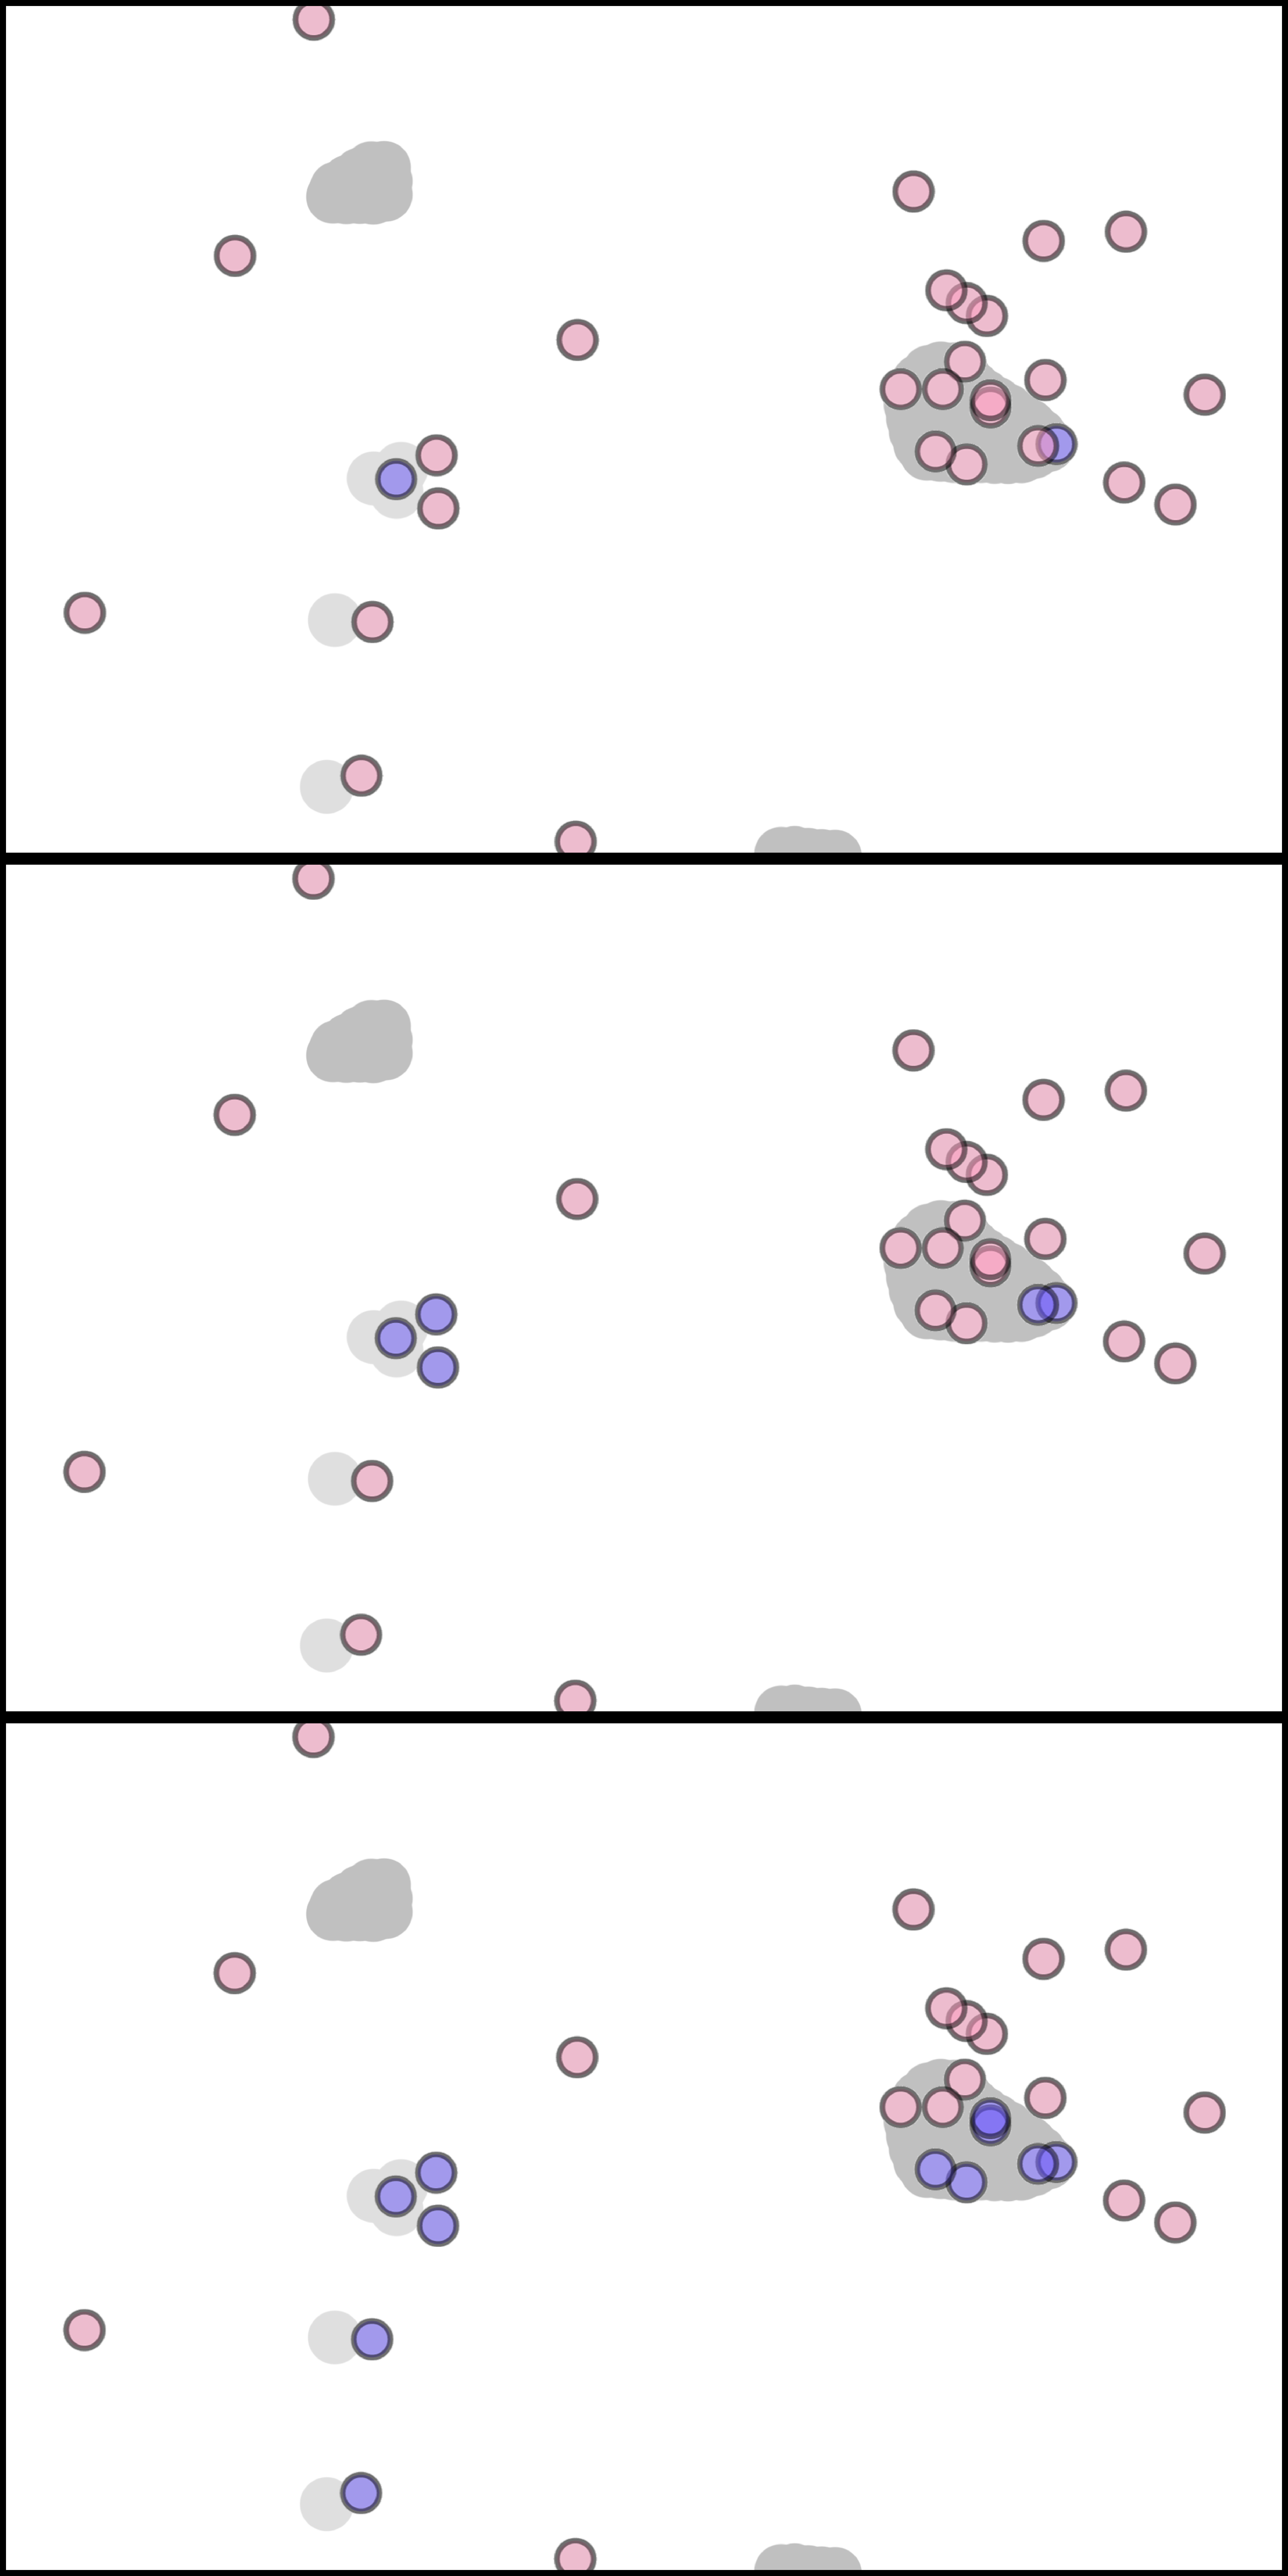
\includegraphics{figures/expansion-v} 

}

\caption{Example expansion over time from 2014 to 2016 (top to bottom) using fake data. Blue dots denote stores with Double Up, pink dots denote without. Gray sectors denote higher population density. The initial nodes can be seen in the top (2014) frame.}\label{fig:dufb-expansion}
\end{figure}

\subsection*{Selection of Control
Stores}\label{selection-of-control-stores}
\addcontentsline{toc}{subsection}{Selection of Control Stores}

Ideally, all remaining stores would have been available to use as a
control group but the company only approved that data be released for 15
stores. This left the added---and incredibly important---step of
selecting the control stores since the company approved, but did not
explicitly select, the 15 stores.

Selecting the control stores proceeded in two steps. First, stores that
either self-selected or were selected using some unobservable criteria
were matched using \emph{Coarsened Exact Matching} (CEM)
\citep{iacus_causal_2011}. Second, stores assigned Double Up were pooled
with nearby control stores and then scored using a linear probability
model. Each step is explained in detail.

\emph{Step 1: Coarsened Exact Matching}

The 6 stores classified as \texttt{self-selected} or \texttt{unobserved}
(stores \texttt{12} through \texttt{17}; see Table
\ref{tab:store-class}) were compared against all possible control stores
for matches. Matching was done across 5 dimensions: race, income,
population density, store attributes, store EBT sales. One variable per
dimension was selected: percentage of population that is
African-American (zip code level); people per square mile (zip code
level); median income for people who have received SNAP or similar
assistance (zip code level); the number of associates employed in each
store; and the percentage of total stores sales attributed to EBT/SNAP.

Of the 6 stores (stores \texttt{12} - \texttt{17}), only 3 produced
viable matches. However, each of the 3 matched stores had matched to
more than one control stores. The closest stores, by driving distance,
were selected as the tie-breaker for each matched store. Stores were
sufficiently far apart, with very sparsely populated areas between, that
``spill-over'' was considered unlikely. That is, it is considered
unlikely that a shopper near a store without Double Up would opt to
drive 30 or more minutes to shop at the store \emph{with} Double Up.

This left 12 stores to be allotted to the control group and 3 treatment
stores to be effectively discarded.

\emph{Step 2: Scoring via Linear Probability Model}

Assignment to treatment and control can be perfectly determined since we
know and observe the criteria used for assignment: geographic distance
from an initial store (node), SNAP EBT sales rank, and
demographics---specifically population density and percentage
African-American.\footnote{It should be noted that the company did not
  explicitly say population and race were part of the selection
  criteria. Instead, they said something along the lines of ``stores
  serving a similar population as the original stores.''} A scoring
function was created by fitting a linear probability model to all stores
within 140 kilometers of the two initial pilot stores.

\[
\begin{aligned}
  \bm{s}  &= \widehat{P(\mathbf{D} = 1 | \bm{X}, \bm{N})} \\
          &= \mathbf{X} \bm{\hat \beta} + \hat \alpha \mathbf{N} + \left (\mathbf{X} \odot \mathbf{N} \right ) \bm{\hat \gamma}
\end{aligned}
\]

\(\bm{s}\) are the fitted values of the estimated linear probability
model; \(\mathbf{D} \in \{0,1 \}\) is a \(n \times 1\) vector of store
assignments to Double Up; \(\mathbf{X}\) is an \(n \times k\) matrix of
normalized observable covariates that determine assignment;
\(\mathbf{N} \in \{0, 1 \}\) is an \(n \times 1\) dummy vector denoting
the closest pilot store aka ``Node'', where \(0\) is \texttt{Node\ 0}
and \(1\) is \texttt{Node\ 1}. \(\odot\) represents element-wise
multiplication aka ``Hadamard product''.

Stores were sorted by the fitted values of the model, \(\bm{s}\). There
is perfect separation between Double Up stores and those without (see
Figure \ref{fig:score-plot}). Therefore, the top 11 stores by score
value are all Double Up stores. The next 12 stores by score value are
then allotted to the control group.

\begin{figure}
\centering
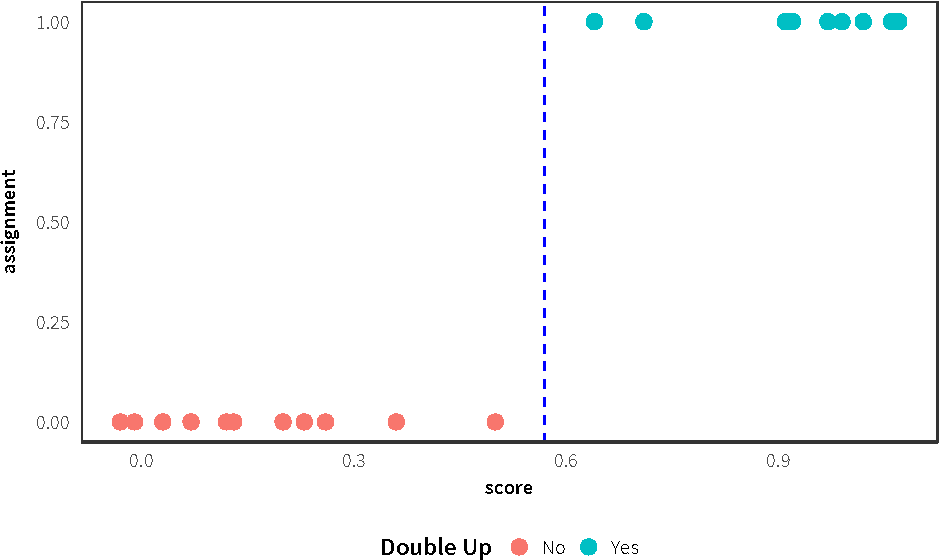
\includegraphics{noriega-prospectus-draft_files/figure-latex/score-plot-1.pdf}
\caption{\label{fig:score-plot}Store Score vs Double Up Assignment}
\end{figure}

\subsection*{Motivation for Matching}\label{motivation-for-matching}
\addcontentsline{toc}{subsection}{Motivation for Matching}

Not all treated stores will be matched to a control. As mentioned, this
is due to the nature of how the 17 treated stores were selected. The
parent company intentionally selected stores with some of the highest
EBT (aka SNAP Electronic Benefit Transfer (EBT) Card) sales that were
also within relatively similar geographic locations. This reduced the
burden of advertising and implementing DUFB for The parent company. The
unfortunate downside of this implementation is that it effectively
removed any likely matches for treated stores located in the most Urban
areas (e.g.~Grand Rapids and Battle Creek).

Here is an example to illustrate why it is infeasible to matching all
treated stores and instead expand selection algorithmically on
observables. If we calculate the percentage of the population by
\emph{zip code} that is African American then split the data into
treatment and control groups, we get the following:

\begin{verbatim}
#> Difference in Means (Treated - Control) = 7.848600
\end{verbatim}

\begin{verbatim}
#> 
#> Population, % Black (Treated, Top 10):
\end{verbatim}

\begin{verbatim}
#>  [1] 26.060929 21.945444 19.790582 18.880000 18.688795 14.693513 11.857163
#>  [8]  8.531952  5.644237  5.644237
\end{verbatim}

\begin{verbatim}
#> 
#> Population, % Black (Control, Top 10):
\end{verbatim}

\begin{verbatim}
#>  [1] 8.575720 8.141256 7.271242 5.057010 4.613969 4.374678 3.256329
#>  [8] 2.955071 2.676733 2.593660
\end{verbatim}

What these results tell us is how potentially distinct the populations
are within the zip codes containing the treated stores. Sorting
population percentages in descending order, no good match exists within
the control stores for the top 7 treated stores. One variable is the
simplest case; matching only gets more difficult as one brings in more
variables to match.

Considering the separation between some of the treated stores and all of
the control stores, it was prudent to rethink the store selection and
matching strategy.

It must be noted that matching is not a necessary step during every
design phase. It is, in large part, a way to hedge against the
possibility that merely selecting the next top 15 stores by EBT sales
could sour the estimates. Matching a smaller set of treatment stores
against a larger pool of controls can often produce estimates less
sensitive to even the smallest changes in some model specifications
\citep{imbens_causal_2015}. However, other models and tools (like
regression) are in relatively unperturbed by a lack of design-phase
matching, but still benefit from having a larger sample size
\citep{angrist_mostly_2008}.

\subsection*{Matching Details}\label{matching-details}
\addcontentsline{toc}{subsection}{Matching Details}

Like most data-dependent endeavors, the most tedious part of matching
the stores was obtaining enough variables. Once enough data were
obtained, variables were selected on how best they captured data from
the following dimensions:

\begin{itemize}
\tightlist
\item
  Demographics (e.g.~race)
\item
  Income/wealth
\item
  Population density (e.g.~urban vs rural)
\item
  Store attributes
\item
  Store EBT sales
\end{itemize}

One may assume that more variables makes matching easier. This is only
true insofar as it provides one with a large pool of options. It is
still necessary to carefully select how many variables one is using
because matching becomes more and more difficult with each added
variable used. This is especially true with a small sample size.

The matching covariates that were finally selected are:

\begin{itemize}
\tightlist
\item
  \texttt{pct\_black} : Percentage of population that is black (zip code
  level)
\item
  \texttt{dens\_pop} : The population density (people per square mile,
  zip code level)
\item
  \texttt{income\_p50\_snap\_yes} : Median income for people who have
  received SNAP or similar assistance (zip code level)
\item
  \texttt{store\_n\_associates} : The number of associates employed in
  each store.
\item
  \texttt{ebt\_sales\_pct} : Percentage of total stores sales attributed
  to EBT/SNAP.
\end{itemize}

~

\textbf{Results of Match}

\begin{table}

\caption{\label{tab:match-results}CEM Match Matrix}
\centering
\begin{tabular}[t]{lrr}
\toprule
  & G0 & G1\\
\midrule
All & 44 & 17\\
Matched & 14 & 3\\
Unmatched & 30 & 14\\
\bottomrule
\end{tabular}
\end{table}

\texttt{G0} represents the ``control'' group and \texttt{G1} represents
the ``treated'' group. One can observe that 3 ``treated'' stores were
matched to 14 ``control'' stores. Each of the 3 treated stores was
matched to its closest control store by driving distance.

\textbf{Covariate Cut-points}

The CEM procedure depends heavily on the ``cut-points'' selected for
each variable. This is akin to setting the cut-off points when turning a
continuous variable into a categorical variable. For example, when
converting income values from dollars into \texttt{low-}
\texttt{middle-} and \texttt{high-income} groups, at least 4 cut-points
are required (2 of which are the maximum and minimum). What the other 2
cut-points are will greatly affect the match. This leads to the
question, for example, should the cut-points be \texttt{25000} and
\texttt{100000} or perhaps the median and the top 10\%?

For the matches produced, the following cut-points were created.

\begin{verbatim}
#> $pct_black
#> [1]  0  2 10 40
#> 
#> $dens_pop
#> [1]    0  200 1000 5000
#> 
#> $ebt_sales_pct
#> [1] 0.00 1.65 3.00 5.00
#> 
#> $store_n_associates
#> [1]  20  40  60  80 130
#> 
#> $income_p50_snap_yes
#> [1] 12000 18000 25000 40000
\end{verbatim}

Understanding why is best explained using a visualization. Below are
graphs of the variables \texttt{pct\_black} and
\texttt{income\_p50\_snap\_yes} with their corresponding cut-points. The
aim of each cut-point is to balance the creation of reasonably sized
partitions while still marking obvious shifts in the underlying
distribution.

For example, in the first plot (\texttt{pct\_black}), there are clearly
points where the slope dramatically increases --- and then spikes --- in
the percentage of African Americans. But in the second plot, the slope
is more gradual, so the partitioning is aimed more at getting relatively
balanced groups.

\includegraphics{noriega-prospectus-draft_files/figure-latex/unnamed-chunk-7-1.png}

\includegraphics{noriega-prospectus-draft_files/figure-latex/unnamed-chunk-8-1.png}

\newpage

\hypertarget{methods-1}{\section*{Methods}\label{methods-1}}
\addcontentsline{toc}{section}{Methods}

\subsection*{Set up}\label{set-up}
\addcontentsline{toc}{subsection}{Set up}

Recall the research question of interest---whether the DUFB incentive
increases spending on fresh fruits and vegetables (FV) within stores
participating in the program. The outcome variable, in this case, is
total spending on FV.

I've considered other possible values for the outcome variable. For
example, the proportion of dollars spent per transaction or the total
ounces of FV purchased. Each added an extra layer of complication. Using
proportion of expenditure per given transaction would vary wildly,
particularly with small transactions, and would creating two mass points
at zero and one (no FV purchased and only FV purchased). Total ounces
depends on the variable and quality of the data. I cannot be sure the
data received will contain counts or ounces for fresh fruits. Fresh
fruits generally do not have UPC values. Dollars spent (expenditures) on
FV gets to the heart of the question and is the data guaranteed to be in
the data.

Unfortunately, using the total expenditure of FV is complicated by 3
problems.

\begin{enumerate}
\def\labelenumi{\arabic{enumi}.}
\tightlist
\item
  Purchases not linked to customers.
\item
  Outcome Variable with non-trivial amount of zeros (corner solutions).
\item
  Consumers maximize across multiple product types.
\end{enumerate}

The first problem is not specific to the outcome variable. The inability
to link purchases to individuals means I cannot use Panel Data Methods
at the customer level; I will be unable to look at how customers
behavior changes over-time and cannot control for unobserved customer
heterogeneity. I'm instead limited to methods for repeated
cross-sections over-time.

The second and third problems are directly related to the preferred
outcome variable. I anticipate a non-trivial amount of zeros because I
expect to observed a large fraction of transaction where no FVs are
never purchased. Likewise, FV expenditures are often a part of a basket
of goods. Just as I anticipate a non-trivial amount of zeros, I also
anticipate that FVs are not purchased independently of other goods. When
spending their money, consumers optimize expenditure across a large set
of options. This optimization is also complicated by the first problem
(cannot link) but I will go into more details later.

\subsection*{Methods Overview}\label{methods-overview}
\addcontentsline{toc}{subsection}{Methods Overview}

\textbf{Difference-in-Difference-in-Differences}

I want to measure the difference in SNAP EBT dollars being spent or
redeemed on fresh produce. If the incentive is working, then I should
see in increase in SNAP EBT dollars spending on fresh produce within
stores implementing the DUFB incentive. I do not think it is enough to
assume the DUFB incentive, if effective, will be measurable without
considering heterogeneity. That is, if a store's implementation of DUFB
affects individual behavior, the effect could be hard to measure if
measured across the entire distribution of FV purchases, instead of the
subset of SNAP EBT dollars spent.

The Difference-in-Difference-in-Differences (DDD) regression is a
fitting framework if I expect the SNAP population that patrons DUFB
(experimental) stores to be systematically different from the SNAP
population that patrons the non-DUFB (non-experimental)
stores.\footnote{See \citet{wooldridge_econometric_2010} for more
  details. I'm assuming familiarity with the DDD model.} Differencing
along time, store experimental group, and the type of transaction (SNAP
or not) will reasonably capture any systematic differences.

This is unfortunately complicated given that I cannot link transaction
to individuals. But I can tell if a purchase was made with SNAP EBT
dollars or that it redeemed DUFB points. This is enough to split
transactions into SNAP/DUFB-redeemed versus other standard transactions.
This provides a way of grouping to perform a DDD.

Any model like DDD that is estimate via OLS, however, ignores the second
and third problems. I think it is prudent to consider consumer choice
behavior and the mechanisms that generate zero-expenditures. Numerous
demand models exists for cross-sectional data that, with a few
assumptions (like each transaction represents a distinct individual),
may better estimate the impact of the DUFB incentive than straight OLS.

There is a vast literature on consumer purchasing behavior aka choice
models (see \citet{train_discrete_2009} for an introductory overview).
Multiple-discrete choice models, in particular, have become popular
given the increased availability of transaction-level (scanner) data
\citep{dube_multiple_2004, hendel_estimating_1999}. Multiple-discrete
choice models, however, are too product-specific. It is not important
for me to model which brand and quality of bananas or carrots were
purchased. What is important to me is how much was spent on bananas,
carrots, and other fruits and vegetable types versus other non-FV types.
Remember, my outcome variable is expenditure on \emph{total} FV
spending. I'm far more concerned about whether or not consumers are
observed buying \emph{any} FV than I am with the exact types. That said,
expenditure on non-FV is also important. \emph{Therefore, what is needed
are model framework flexible enough to handle a continuous outcome
variable with a non-trivial amount of zeros (corner solutions) and
multiple types of goods.}

\textbf{Continuous Outcome Variables and Corner Solutions}

Corner solutions for expenditures can occur for various reasons.
\citet{pudney_modelling_1989} covers three of the most likely mechanisms
producing ``true'' zeros in cross-sectional data. The first is that the
data was gathered in too short a period of time for the purchase to
occur. This problem is far more common in cross-sectional data of
infrequently purchased goods (i.e.~durable goods like cars or
refrigerators). The second is due to a supply side factor the customer
has no control over. For example, there could be a shortage of FVs or
none are available. Imagine searching for FV purchases in collection of
convenience store data. Many zeros would exists because some convenience
stores do not sell FVs. The third zero results from a customer's
decision as a function of prices, preferences, and income constraints. A
zero is perhaps observed because FVs are too expensive and the customer
can get larger quantities of other, equally or more preferred, foods for
the same price.

I expect first mechanism could apply to food purchases under specific
circumstances. If data are left disaggregated or the period of
observation is shrunk substantially, zeros for FVs will exists due to
infrequency of purchase. For example, customers that make frequent trips
to the store may not always buy FVs. A cross-section of data from one
day may have a non-zero FV value for the customer but zero the next. The
third mechanism applies very naturally to the grocery store environment
(classical utility theory). The second will require further
verification. I do not expect to find out that there were shortages of
FVs in the stores observed, but I could be wrong.

\citet{humphreys_dealing_2013} and \citet{carlevaro_multiple_2016}
discuss cross sectional models that accommodate corner
solutions---Tobit, \emph{Two-Part}, and \emph{Hurdle} models,
specifically.\footnote{\citet{wooldridge_econometric_2010} does not
  appear to differentiate between ``Two-Part'' models and ``Hurdle''
  models. I will use it following \citet{humphreys_dealing_2013}
  language, which does.} The classic ``corner solution'' regression
model is the Tobit model. Corner solutions are utility maximizing and no
assumptions are made about the decision not to purchase/consume. In
contrast to the Tobit model, the decision to participate in consumption
is explicitly formulated in the Two-Part and Hurdle models.
Participation is the ``first hurdle'', the amount purchased/consumed is
the ``second hurdle''.

In the ``Naive'' Two-Part model, the decision to buy is estimate
separately and sequentially from how much (amount) to buy; Probit is
used to estimate the decision-to-buy process and OLS is used to estimate
the amount purchased. The Double Hurdle model estimates both these
decision simultaneously via maximum likelihood. The full Double Hurdle
model allows for correlation between the error terms in the decision and
amount/consumption equations \citep{jones_note_1992}. Imposing the
assumption that unobservable factors between the decision and amount
decisions are uncorrelated reduces the full ``Jones'' Double Hurdle to
the ``Cragg'' model \citep{cragg_statistical_1971}.

It is unclear to me if Two-Part or the Double Hurdle models that
formalize ``participation'' are necessary when considering FV purchases.
This makes more intuitive sense for something like cigarette or alcohol
consumption, where zero-expenditure can be the result of abstention or
price/income constraints.\footnote{See \citet{garcia_alternative_1996}
  and \citet{aristei_cohort_2008} for abstention-style hurdles.} There
are, after all, consumers who will never consume cigarettes or alcohol,
even if free (abstention). But I'm not sure if an abstention mechanism
is reasonable when considering FV purchases. Do consumers really opt out
(or abstain) form buying FVs altogether?

An infrequency of purchase mechanism for FVs, however, seems more
reasonable. \citet{deaton_statistical_1984} introduced this mechanism as
an expansion to the Tobit model. This Double Hurdle has been used to
model infrequent purchases of butter, pork, and prepared meals
\citep{yen_modeling_1995, su_microeconometric_1996, newman_double-hurdle_2003}.
I find it reasonable to expect that, for any given daily cross-section
of data, some of the zeros observed will be due to infrequent purchase
of FVs.

It's worth noting the general increased popularity of Hurdle models as
alternatives to Tobit, and other related models, like Adjusted Tobit and
Heckit models. There is a long existing debate over which models perform
better, with most of the criticism falling on Tobit. Monte Carlo
comparison under different error distributions and exclusion
restrictions find Hurdle models consistently out performing Tobit and
Heckit models, both in model fit and coefficient bias
\citep{hay_ordinary_1987, manning_monte_1987}. Monte Carlo studies have
also been used to defend both approaches, encouraging a more flexible,
case-by-case approach on choosing the appropriate model
\citep{leung_choice_1996, dow_choosing_2003, madden_sample_2008}. But
applied work in the applied social science, like health care expenditure
and consumer purchases, generally tend to favor use of Hurdle models
over Tobit or Heckit models
\citep{yen_working_1993, smith_tobit_2003, stewart_tobit_2013}.

\textbf{Multiple Goods}

The limitation of Tobit and other hurdle models is the estimated demand
of a single good. Ideally, expenditure on different types of goods
better captures the decisions and purchasing behavior of customers
within a grocery store. That is, instead of collapsing all expenditure
on FVs into one outcome variable, the model would allow for customers to
optimize across \emph{multiple} goods of different types, while also
allowing corner solutions. Multiple discrete choice models allow the
purchase of multiple types of goods, but do not capture the intensive
margin (the amount) of the good purchase/consumed.

\citet{dubin_econometric_1984} construct a \emph{discrete-continuous}
model were consumers can select from multiple goods/options but that
they are mutually exclusive, perfect substitutes. The \emph{discrete}
component of the model captures the decision to buy a non-zero amount;
the \emph{continuous} part captures the amount
purchased/consumed/utility acquired. The mutually exclusive, perfect
substitute condition, however, means that one cannot be observed
buying/consuming more than one good/option.

For any observed trip to the store, zero-expenditure in FV implies
non-zero expenditure for some non-FV. Ignoring this seems unwise and I
plan, at a minimum, to implement a model optimize along two
dimensions---FV and non-FV. The best model I've found is the
\emph{multiple} discrete-continuous model extreme value (MDCEV) model
introduced by \citet{bhat_multiple_2005}. MDCEV is an extension of the
Kuhn-Tucker based model developed by \citet{wales_estimation_1983}.
MDCEV allows non-zero consumption across multiple goods.
\citet{kim_modeling_2002} solved the intractability of the
\citet{wales_estimation_1983} model. \citet{bhat_multiple_2005}
simplified both to be more realistically applicable.

In the next subsection, I will formally introduce the different modeling
structures I intend to use in my paper. I will first introduce the DDD
framework were estimation via OLS is sufficient. I then expand from OLS
to Tobit and other Hurdle models before expanding into the more complex
MDCEV model. The share goal, across all models, is the best possible
measurement of the impact the DUFB incentive has on fruit and vegetable
expenditures between participating and non-participating stores.

\begin{center}\rule{0.5\linewidth}{\linethickness}\end{center}

\subsection*{Difference-in-Difference-in-Differences
(DDD)}\label{difference-in-difference-in-differences-ddd}
\addcontentsline{toc}{subsection}{Difference-in-Difference-in-Differences
(DDD)}

I observe transaction \(i=1,...,L\) in store \(j=1,...,N\) across
\(t=1,...,T\) days. Let \(y_{ijt}\) be total FV expenditures for
transaction \(i\) in store \(j\) on day \(t\). The DDD regression is

\[
\begin{aligned}
y_{ijt} &= \alpha_0 + \alpha_1 dE_j + \alpha_2 dS_i  + \alpha_3 dE_j \cdot dS_i \\& \quad + \theta_1 dP_t + \theta_2 dP_t \cdot dE_j + \theta_3 dP_t \cdot dS_i \\
& \quad + \delta dE_j \cdot dS_i \cdot dP_t + \bm{x'}_{ijt} \bm{\beta} + \lambda_t + \epsilon_{ijt}
\end{aligned}
\]

where \(dE_j\) represents store assignment to experimental group,
\(dS_i\) represents a SNAP or SNAP related transaction (target group),
and \(dP_t\) represent the treatment period, August - December.
\(\lambda_t\) captures daily (time) effects and \(\bm{x'}_{ijt}\) is a
vector of observable characteristics about transaction \(i\) in store
\(j\) on day \(t\). The coefficient of interest is \(\delta\).
\(\epsilon_{ijt}\) are idiosyncratic errors at the transaction level.

Again, I do not observed individuals, only transactions. Yet I think it
reasonable to assume that the structure of daily transaction data more
closely resembles that of repeated cross-sections than of panel data.
Assuming it was possible to link individuals to purchases and build
panel data. The same individual would likely observed
\emph{sporadically} within in a given month. That is, were this to be
panel of the same \(N\) individual shoppers across \(T\) total days,
many---if not most---of those days would have missing data. There would
certainly be shoppers observed multiple times per week, but I expect
such shoppers to be rare. I certainly would not expect to have a
balanced panel and no shopper would be observed all 365 days.

I therefore find it reasonable to treat each day of observed data as a
single independent cross-section of \(L\) transactions generated by an
unknown \(N \le L\) individuals across \(J\) many stores. Aligned
sequentially, these form a repeated cross-sections over-time. Each
transaction also falls naturally into a cluster---the store where it
occurred---that is time-invariant and determined prior to the data being
collected.

The model DDD model above can be improved by introducing store effects.
These effectively capture experimental assignment and all other
time-invariant store-level characteristics. The \(dE\) dummy, for
example, drops out. The notation can also be cleaned up by condensing
the others dummies, emphasizing only variation. The spruced up model is

\begin{equation}
y_{ijt} = \gamma_j + \lambda_t + \phi_0 D_i + \phi_1 D_{ij} + \phi_2 D_{it}+ \phi_3 D_{jt} + \delta_t D_{ijt} + \bm{x'}_{ijt} \bm{\beta} + \epsilon_{ijt}
\label{eq:ddd}
\end{equation}

where \(\gamma_j\) now represents store effects, \(dS_i \equiv D_i\),
and the remaining dummy variables \(D_{ij},~D_{jt},~D_{it},~D_{ijt}\)
represent the dimensions along which they vary---\(i\) transaction type
(SNAP or not), \(j\) store experiment group, and \(t\) day during DUFB
treatment period (August - December). To capture more detail than just
the average, \(\delta_t\) is allowed to vary by day.

\textbf{Unobserved Effects}

I still do not know what the transaction characteristic variables will
be and hence do not know what variables go into \(\bm{x'}_{ijt}\). I do
know, however, that without panel data, I have no methods for dealing
with unobserved individual effects. That is, some unobserved individual
effect \(c_i\) likely exists such that \(e_{ijt} = c_i + u_{ijt}\) where
\(\exists t \ni E[\bm{x'}_{ijt}c_i] \ne 0\). In short, my estimates will
be biased due to an omitted variables problem.

I'm am still thinking about how I can capture part of the unobserved
individual effect \(c_i\). I am open to suggestions.

\begin{center}\rule{0.5\linewidth}{\linethickness}\end{center}

\subsection*{Tobit and other Hurdle
Models}\label{tobit-and-other-hurdle-models}
\addcontentsline{toc}{subsection}{Tobit and other Hurdle Models}

Calculating fruit and vegetable expenditures, \(y_{ijt}\), for each
transaction will result with a non-trivial amount of zeros. These zeros
are not ``censored'' values in the Heckman selection problem sense. They
are genuine zeros aka ``corner solution''. But the mechanisms behind the
zeros is unknown.

\textbf{Tobit Model}

The Tobit model is agnostic to the economic mechanism generating corner
solutions. It is the basic approach when little else is known other than
the decision not to purchase fruits and vegetables is resulting in
zero-expenditures. The basic structure is

\[
\begin{aligned}
y^* &= x'\beta + u \\
y &= max(0, y^*)
\end{aligned}
\]

where \(y^*\) is a latent variable and \(y\) is observed. Tobit can be
generalized beyond requiring homoskedastic error terms but requires
normality. This is important because error terms in repeated cross
sectional data are assumed independent \emph{not} identically
distributed. In other words, heteroskedastic. Other than error term
specifications, any additive and linear-in-parameters regression can
estimated using Tobit. In other words, I can set \(y^*\) equal to
equation \eqref{eq:ddd}.

For details on the likelihood functions, see \citet{amemiya_tobit_1984}.

\textbf{Hurdle and (Naive) Two-Part Models}

Hurdle models generally have two parts (i.e. ``Double'' Hurdle)---a
decision-to-buy (participate) and the amount to purchase (consumption)
\citep{jones_double-hurdle_1989}. Let \(I^* \in {0,1}\) indicate the
decision to purchase fruits and vegetables and \(y^*\) be the amount of
dollars spent. Both are latent variables. Let \(y\) be observed
expenditures. Formally,

\[
\begin{aligned}
I^* &= z'\gamma + v \\
y^* &= x'\beta + u  \\
y   &= I^* \times max(0, y^*) \\
& \phantom{x}\\
(u,v) & \sim N(0,\Omega) \\
\Omega & = {\left ( 
\begin{array}{cc}
  \sigma^2_{u} & \sigma_{uv} \\
  \sigma_{uv} & \sigma^2_{v} 
\end{array}
\right )}
\end{aligned}
\label{eq:dhurdle}
\]

The \citet{jones_double-hurdle_1989} ``Full'' Double Hurdle model and
the \citet{cragg_statistical_1971} have the same framework. The
distinction is that in the Cragg model assumes no correlation between
\(u\) and \(v\) (i.e. \(\sigma_{uv} = 0\)). The likelihood function for
the Cragg model is, in other words, a simplification of the Jones model.
Formally, the Jones model is

\[
\begin{aligned}
L &= \prod_0 
  \left [
    1 - \Phi 
    \left ( 
      \frac{z'\gamma}{\sigma_v},
      \frac{x'\beta}{\sigma_u},
      \rho
    \right ) 
  \right ] \times \\
& \quad ~ \prod_{+} \Phi
  \left [ 
      \frac{ \left ( 
        \frac{z'\gamma}{\sigma_v} + 
        \rho(y^* - x'\beta) \right )}
         {\left ( \sqrt{1 - \rho^2} \right ) } \right ]
\frac{1}{\sigma_u} \phi \left ( \frac{y^* - x'\beta}{\sigma_u} \right )
\end{aligned}
\label{eq:lhurdle}
\]

Once again, setting the DDD to be \(y^*\) is not a problem. The main
problem is determining the participation equation \(I^*\). What factors
variables participation i.e.~the decision-to-buy fruits and vegetables?
Variables about individual characteristics would certainly be helpful
here but that isn't possible. There is clearly some mechanism driving
consumers to buy or not buy fruits and vegetables. The likeliest
candidate is data on \emph{other} products purchased within a given
transaction. The existence of complimentary goods (e.g.~olive oil,
meats, etc) may increase the likelihood of observing FV purchases within
the same trip. The size of the shopping basket likely increases overall
chances of FV purchases. Likely day of the week or week of the month,
since government benefits and pay schedules may increase the chances of
shopping trips in aggregate.

I anticipate estimate both the Jones and Cragg model as a robustness
check. But I do not expect \(Cov(\sigma_u, \sigma_v) = 0\) given I
cannot capture individual effects. Unobserved individual effects likely
affect both participation and consumption. In both equations, individual
effects are absorbed by the error terms, making them correlated by
construction.

I will also estimate a ``Naive'' Two-Part model, where the participation
and consumptions equations are estimate independently from the other
(Probit + OLS). Again, just another comparison point.

\textbf{Multiple Discrete-Continuous Extreme Value Models}

The \citet{bhat_multiple_2005} Multiple Discrete-Continuous Extreme
Value (MDCEV) framework allows for choice along a vector of non-mutually
exclusive goods. Non-negative consumption is allowed in across all
goods.

I will attempt to use a later iteration of the MDCEV model from
\citet{bhat_multiple_2008}. The distinction that interest me is that the
Bhat (2008) model allows for price variation across goods and explicitly
formulates the Kuhn-Tucker constraints using expenditures. The
econometric model is as follows.

Utility from purchasing vector of goods \(\bm(x) = (x_1, x_2,...,x_k)\)
is defined as

\[
\begin{aligned}
\tilde{U} &= \sum_k \frac{\gamma_k}{\alpha^*_k} \psi(z_k, \epsilon_k)
  \left [ 
    \left (
      \frac{y_k}{\gamma_k p_k} + 1
    \right )^{\alpha_k} - 1
  \right ] \\
\psi(z_k, \epsilon_k) &= exp(z'_k\beta + \epsilon_k)
\\
\sum_k p_k &= Y
\end{aligned}
\]

where \(z_k\) is a vector of attribute variables about product \(k\) and
of the consumer, \(y_k\) is expenditure on product/good \(k\), \(p_k\)
is the price, and \(Y\) is total expenditure on basket of goods
\(\bm(x)\). \(\epsilon_k\) are idiosyncratic shocks with an
extreme-value distribution. To understand the role of \(\psi_k\),
\(\alpha_k\) and \(\gamma_k\), see \citet{bhat_multiple_2008} for
details.

Using the first good as a reference group, the KT conditions that solve
the optimal expenditure problem (the Lagrangian above) are

\[
\begin{aligned}
V_k^* + \sigma \epsilon_k &= V_1^* + \sigma \epsilon_1 \text{ if }
  y_k^* > 0 (k = 2,3,...,K) \\
V_k^* + \sigma \epsilon_k &< V_1^* + \sigma \epsilon_1 \text{ if }
  y_k^* = 0 (k = 2,3,...,K), \text{ where } \\
V_k^* &= \sigma z'_k \beta + \sigma (\alpha_k - 1)
  \text{ln} \left ( \frac{y_k}{\gamma_k p_k} + 1 \right ) - \text{ln} p_k
\end{aligned}
\]

where \(V_k\) is identified only when \(\alpha_k\) or \(\gamma_k\) is
fixed (both terms estimate related ``satiation'' behaviors). See
\citet{bhat_multiple_2008} (equations 18 and 19) for the Jacobian and
closed form expression for the probability of spending \(y_k^*\).
Example likelihood function to solve the equation for \(i=1,...,L\)
transaction (or \(N\) individuals) in a given cross-section can be found
in \citet{bhat_multiple_2005} (equation 18) and
\citet{bhat_household_2006} (equation 8).

\textbf{Expected Challenges with this Model}

Despite the theoretical advantages of the MDCEV framework
(i.e.~optimization over multiple goods allowing corner solutions), there
are a few challenges I anticipate with using the MDCEV framework.

The first is a concern about prices. The most effective way to
incorporate price variation is to make the basket of available goods
equal to the full universe of observed products. This would likely be
huge. The MDCEV framework is flexible enough to do it, but my fear is
that it will lead to some difficulties in interpretation. In reality,
however, I don't care as much about expenditure at the product level as
much as I do about expenditure on particular types. That is, I care more
about spending on FVs versus non-FVs. Therefore, at the simplest level,
my vector of possible goods would be just 2. However, how would I price
FV versus non-FV? I could construct a price index for just those two
groups but it would combine far too many distinct food types to be
reasonable. Moving towards something like having between 20 to 40
general food categories seems like better approach. For example,
\citet{harding_effect_2014} estimate the prices for 33 different product
groups by using the Stone price index, which depends only on observable
price values.

The second concern is programming related. There are no available
packages that implement the MDCEV package. I would have to adapt the
GAUSS code provided by Bhat on his website in order to get the model
running. This isn't a concern about being able to do it as much as the
amount of time it would require to learn/understand GAUSS in order to
implement it in R or Python.\footnote{It looks like some folks at the
  company \href{http://www.mobilityanalytics.org}{Mobility Analytics}
  have started, which is very promising.}

\newpage

\begin{center}\rule{0.5\linewidth}{\linethickness}\end{center}

\textbf{!!BELOW HERE BE DRAGONS (SUPER WORK IN PROGRESS)!!}

\subsection*{Regression Discontinuity
(RD)}\label{regression-discontinuity-rd}
\addcontentsline{toc}{subsection}{Regression Discontinuity (RD)}

I will also perform a secondary Regression Discontinuity (RD) Design
analysis.

In the \protect\hyperlink{store-selection-1}{Store Selection} section, I
discussed the construction of the score function
\(\bm{s} = \widehat{P(\mathbf{D} = 1 | \bm{X}, \bm{N})}\). The score of
each store can be determined via observable data,
\(s_{j} = \widehat{P(D_{j} = 1|\bm{x}_{j}, n_{j})}\). These scores, when
ordered, produced perfect separation between experimental stores and
control stores (see Figure \ref{fig:score-plot2}).

An RD design requires a \emph{running variable} where, above some value
\(c\), the probability of being assigned to the experimental group is
\(1\). Assume I make the score function \(\bm{s}\) my running variable
such that \(D_{j} = \bm{1}[s_{j} \ge c]\).

In my case, assignment \(D_{j}\) is determined by \(s_{j}\) by
construction. Recall that \(s_{j}\) is a function estimated on
observable covariates. These are the same observable covariates the
company used to determine assignment for a subset of stores. I used a
linear probability model to estimate the score function and the
estimated model perfectly predicted assignment. I then ordered stores by
their score value and selected the next 12 unassigned stores.

This problem is that I do not actually know \(c\). I only know that
\(c \in (0.50, 0.64)\). The light gray band in Figure
\ref{fig:score-plot2} displays the possible values of \(c\). The
problem, in essence, is that I do not have---and never will
have---enough stores, so I'm lacking density around where the separation
occurs.

\begin{figure}
\centering
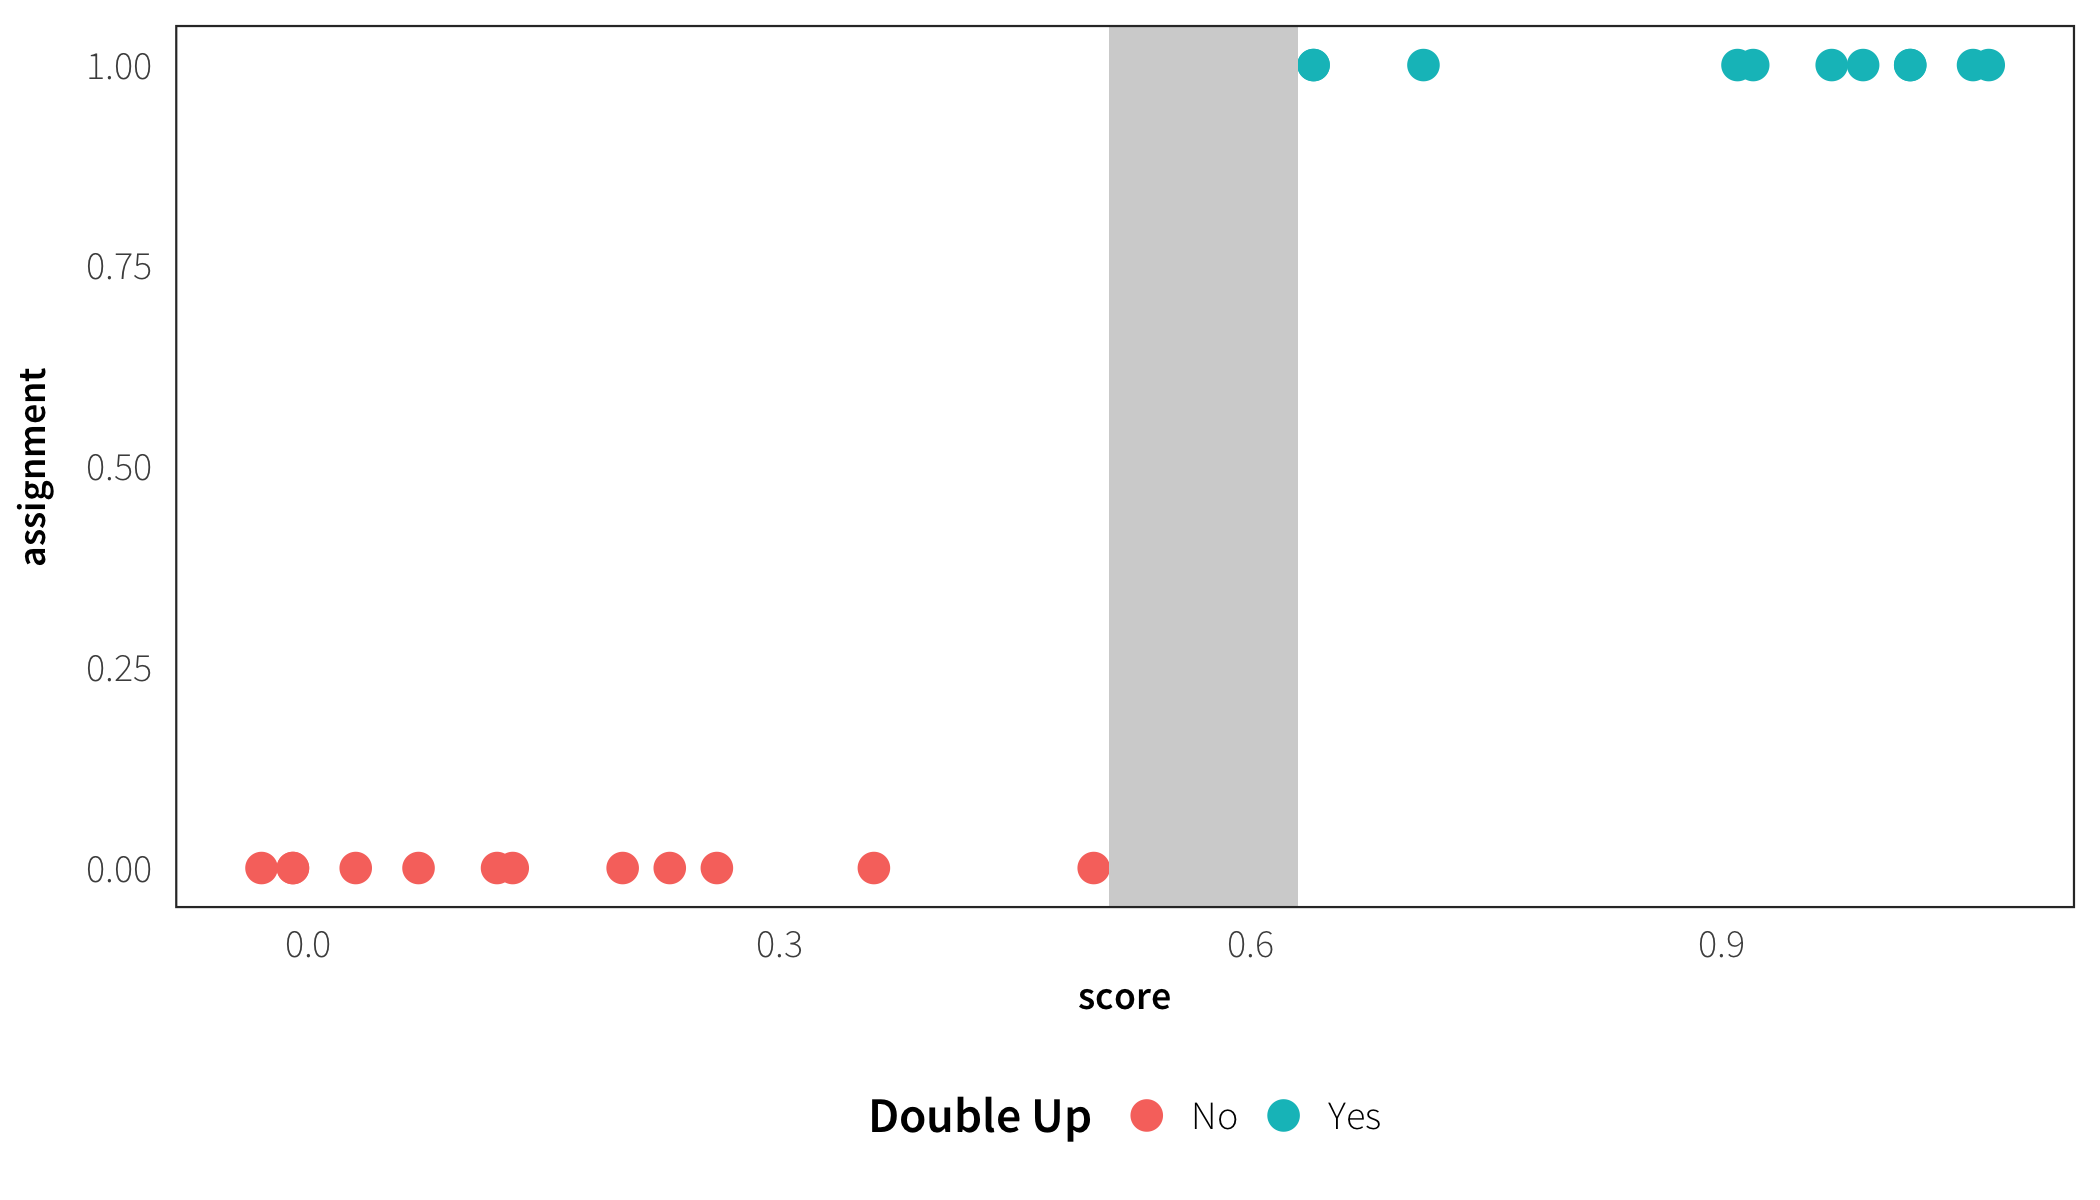
\includegraphics{noriega-prospectus-draft_files/figure-latex/score-plot2-1.pdf}
\caption{\label{fig:score-plot2}Store Score vs Double Up Assignment with
Uncertainty Band (light gray)}
\end{figure}

I propose to estimate the RD design using various values of \(c\). The
perpetual gap means any model estimate to the left or right of some
\(c_0 \in (0.50, 0.64)\) will have to be extrapolated up to \(c_0\).

\textbf{Set-up}

The outcome of variable, as before, is \emph{the total daily amount of
dollars spent on fruits and vegetables per store transaction}. I decided
on using days as the unit of observation to increase the sample amount
of data for estimating. I expect there to be enough transactions per day
for this to be possible. The time frame will be August - December
(months \(8\) - \(12\)) of 2016, when the DUFB incentive is place. Only
SNAP transactions will be considered and transactions will be pooled.
Given that stores may vary in sales volume sold, I may divide by total
SNAP dollars spent so that the outcome variable is instead a proportion.
In total, there will be \texttt{11} treated (experimental) stores and
\texttt{12} control stores.

Let \(y_{ijt}\) represent the outcome variable where \(i=1,...,K\),
\(j=1,...,N\) denotes stores across \(t=1,...,T\). Let \(c\) denote the
cutoff; \(s_{j}\) the score computed for store \(j\); and \(D_{j}\) the
assignment variable. Each draw (or row) of data for store \(j\) is a
vector \((y_{jt}, s_{j}, D_{j})\)corresponding to a single day.
\(\lambda_t\) are time effects and \(u_{jt}\) is an idiosyncratic store
level error term.

The RD model I propose follows the setup of \citet{lee_regression_2010}
(section 4.3):

\[y_{jt} = \alpha + \lambda_t + \rho D_{j} + \gamma (s_{j} - c) + \delta D_{j}(s_{j} - c) + u_{jt}\]

\textbf{Expected Results}

Plotting RD data and observing a visual gap is standard. The first thing
I would do is plot the outcome variable of interest---total daily
(fraction of) SNAP dollars spent on fruits and vegetables--against the
running variable \(s_j\). A total of \(N \times T\) (23 \(\times\) 153)
data points exists; each value of \(s_j,~j=1,...,23\) will contain
\(T=153\) points.

The graph produced will have more gaps compared to conventional RD
graphs. In more conventional RD graphs, each point represents a single
value for a single person (e.g.~score on an exam), producing more points
along the running variable axis. I do not have enough stores to produce
enough \(s_j\) values for this to be possible. Instead, this RD design
plots multiple points per stores, creating a distribution such that the
mean (or median) value (with some confidence interval) becomes the
fitted values of interested. Estimation wise, this distinction changes
very little; \(E[y_{jt}|s_{j}, D_{j}]\) effectively fits a mean value to
each different store. But graphically, what matters in my RD is the
overlap between distributions before and after the cut-off point.

\bibliography{bib/book.bib}

\backmatter
\printindex

\end{document}
